\documentclass{article}
\usepackage{amsmath}
\usepackage{amsthm}
\usepackage{amsfonts}
\usepackage{amssymb}
\usepackage{bbold}
\usepackage{dsfont}
\usepackage{graphicx}
\usepackage{cleveref}
\usepackage{bm}
\usepackage{booktabs}
\usepackage{siunitx}
\usepackage{xcolor}
\usepackage{pdfpages}
\usepackage[utf8]{inputenc}
\usepackage[english]{babel}
\newtheorem{definition}{Definition}
\newtheorem{example}{Example}
\newcommand{\exP}[1]{\mathrm{e}^{#1}}
\newcommand{\dif}{\mathrm{d}}
\renewcommand{\vec}[1]{\mathbf{#1}}
\newcommand{\pdagger}{{\phantom{\dagger}}}
\newcommand{\state}[1]{\vert #1\rangle}
\newcommand{\cstate}[1]{\langle #1\vert}
\newcommand{\tr}[1]{\mathrm{tr}\left\{#1\right\}}
\newcommand{\trs}[2]{\, \mathrm{tr}_{#1}\{#2\}}
\newcommand{\expc}[3]{\langle #1\vert #2 \vert #3\rangle}
\usepackage[doi=false,url=false,isbn=false,backend=bibtex,style=nature,natbib=true,sorting=none]{biblatex}
\bibliography{bib.bib}
\usepackage{geometry}
\geometry{
	a4paper,
	total={170mm,257mm},
	left=15mm,
	right=15mm,
	top=15mm,
}
\begin{document}
\title{Report 16: Ehrenfest: Variation of vib.-assisted SOC}
\author{Rudolf Smorka}
\maketitle
%\section{Ehrenfest: Variation of vib.-assisted SOC}
The currents through Fransson's model with $L=2\times 4$ sites and $\lambda_1=\SI{5}{\milli\electronvolt}$ are shown in \cref{fig:L2x4_tsoPh5} and for $\lambda_1=\SI{10}{\milli\electronvolt}$ in \cref{fig:L2x4_tsoPh10}. Since there is a significant change of the current even for $\SI{10}{\pico\second}$, calculations for later times are currently running on the cluster.
The spin polarization are compared for varying $\lambda_1$ in \cref{fig:L2x4_tsoPhVar_1,fig:L2x4_tsoPhVar_2}. Note that the sign of $S$ for a certain time period is negative. This is related to the system size/number of sites per turn, as can be seen in \cref{fig:tsoPh0.1_LVar_1,fig:tsoPh0.1_LVar_2}
The time-dependent spectra for the larger $\lambda_1$ are shown in \cref{fig:SpecTD_tsoPh5,fig:SpecTD_tsoPh10}. These plots show also the bias window for comparison of energy scales.

{\color{red} Results for $\varepsilon_0=0$ currently running. Suspecting that the asymmetric voltage bias, as is induced by having a shift by $\varepsilon_0$, leads to the observed spin polarization. This hypothesis is correct. The spin polarization is very small when $\varepsilon_0=0$. Currently running longer times.}

{\color{blue} The main point of the comparison for different $\varepsilon_0$ and different $\lambda_1$ is, that while increasing $\lambda_1$ somewhat increases $S$, but not as much as choosing a proper $\varepsilon_0$. Even with large $\lambda_1$ but $\varepsilon=0$, the $S$ is smaller than with a very weak $\lambda_1$ but non-zero $\varepsilon_0$. I need to understand why this is. Asymmetry of voltage drop? Role of vibrations?}
\begin{figure}[!h]
	\centering
	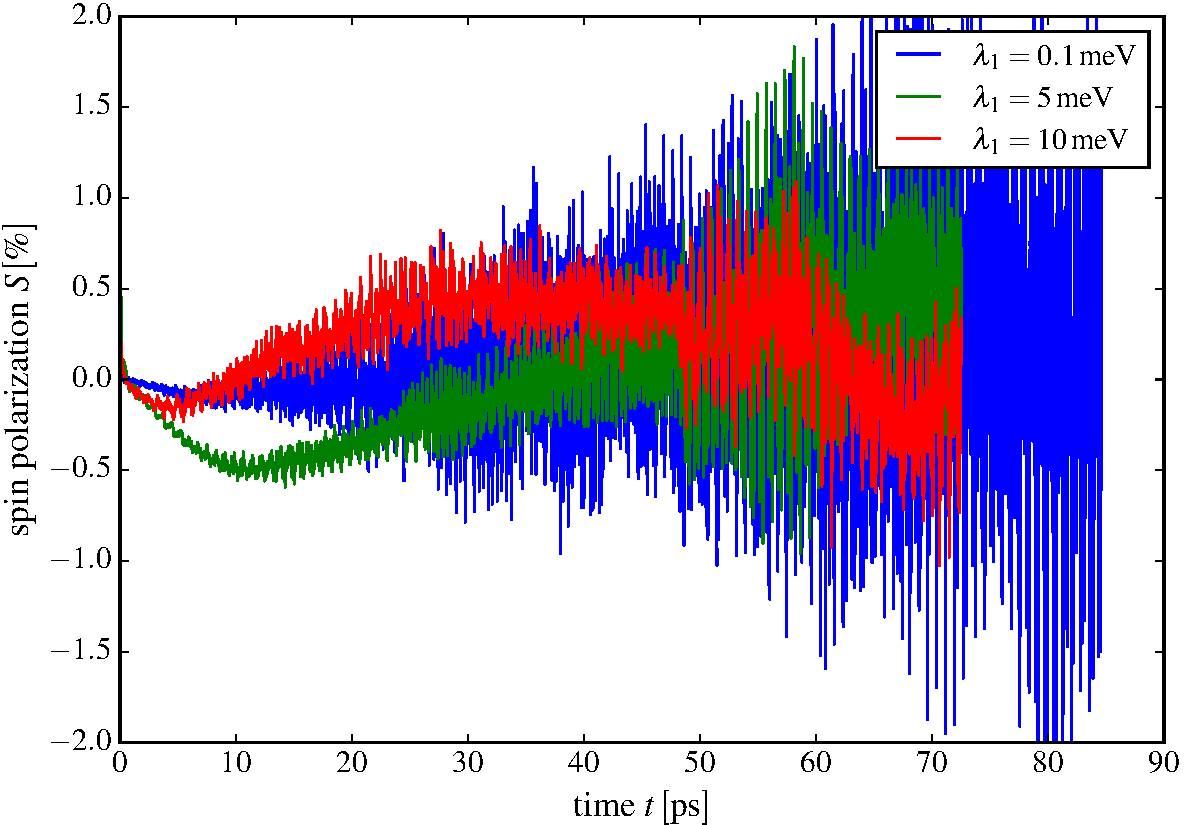
\includegraphics[width=0.45\textwidth]{figs/SpinPolarizations_L2x4_tsoPh_var_V60.pdf}
	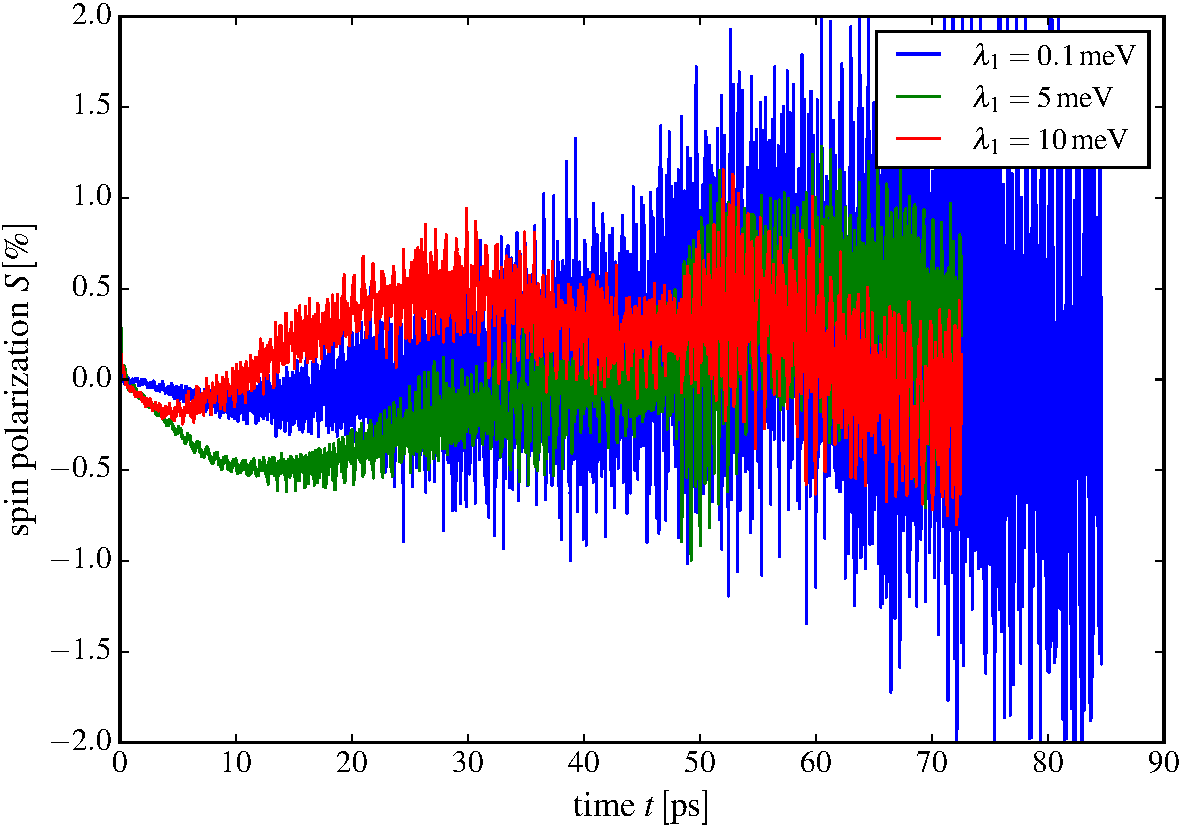
\includegraphics[width=0.45\textwidth]{figs/SpinPolarizations_L2x4_tsoPh_var_V65.pdf}
	\caption{Comparison of spin polarization for varying $\lambda_1$ and $V=\SI{0.48}{\volt}$ (left) and $V=\SI{0.52}{\volt}$ (right). Number of trajectories are 525 ($\lambda_1=\SI{0.1}{\milli\electronvolt}$), up to 20300 ($\lambda_1=\SI{5}{\milli\electronvolt}$) and up to 26300 ($\lambda_1=\SI{10}{\milli\electronvolt}$).}\label{fig:L2x4_tsoPhVar_1}
\end{figure}
\begin{figure}[!h]
	\centering
	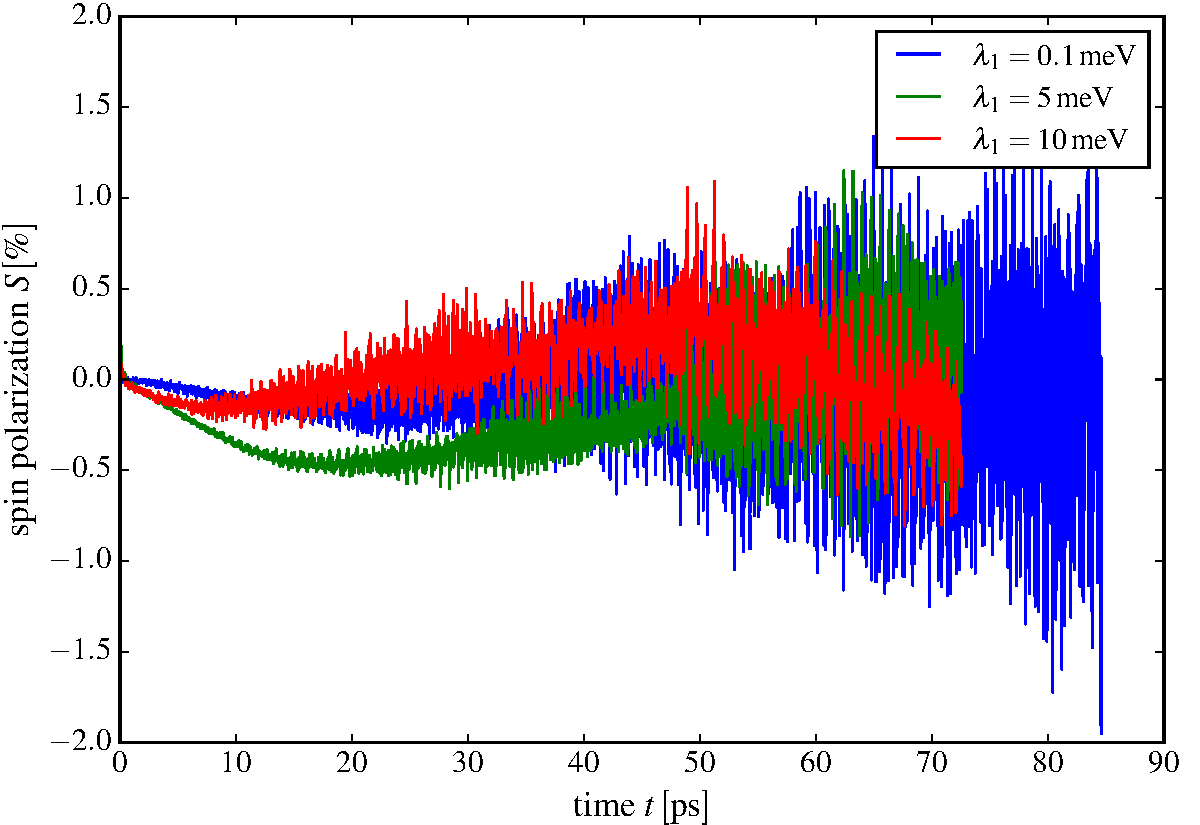
\includegraphics[width=0.45\textwidth]{figs/SpinPolarizations_L2x4_tsoPh_var_V75.pdf}
	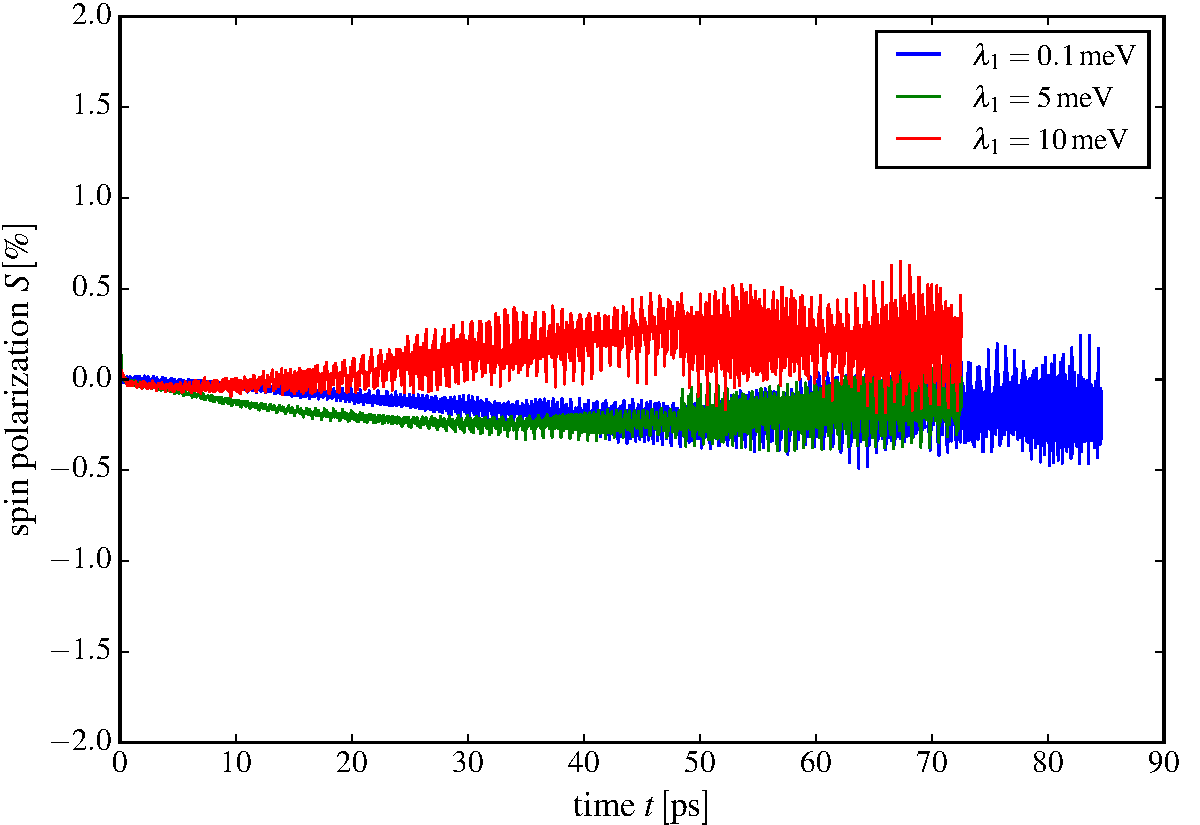
\includegraphics[width=0.45\textwidth]{figs/SpinPolarizations_L2x4_tsoPh_var_V85.pdf}
	\caption{Comparison of spin polarization for varying $\lambda_1$ and $V=\SI{0.6}{\volt}$ (left) and $V=\SI{0.68}{\volt}$ (right).}\label{fig:L2x4_tsoPhVar_2}
\end{figure}
\begin{figure}[!h]
	\centering
	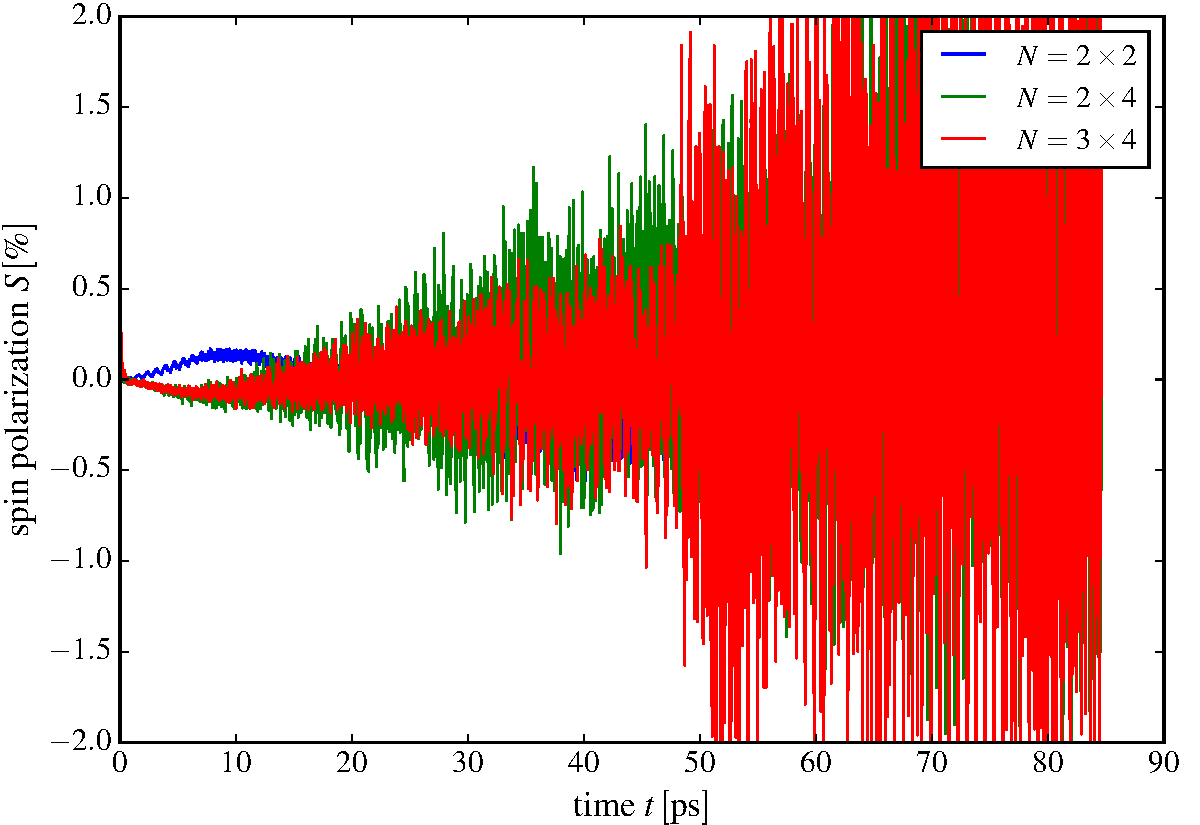
\includegraphics[width=0.45\textwidth]{figs/SpinPolarizations_tsoPh_0.1_N_var_V60.pdf}
	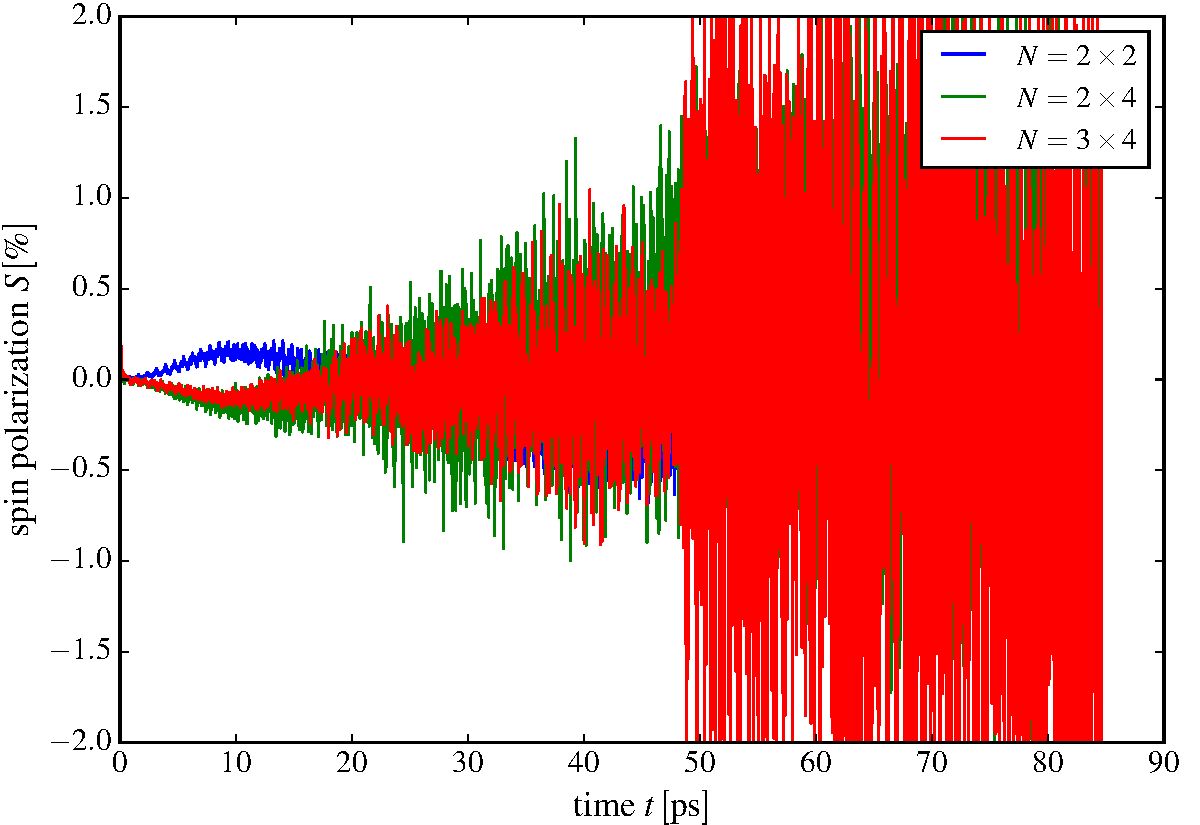
\includegraphics[width=0.45\textwidth]{figs/SpinPolarizations_tsoPh_0.1_N_var_V65.pdf}
	\caption{Comparison of spin polarization for $\lambda_1=\SI{0.1}{\milli\electronvolt}$ and varying system size and $V=\SI{0.48}{\volt}$ (left) and $V=\SI{0.52}{\volt}$ (right). Number of trajectories are 2500 ($L=2\times 2$), 3100 ($L=3\times 4$). }\label{fig:tsoPh0.1_LVar_1}
\end{figure}
\begin{figure}[!h]
	\centering
	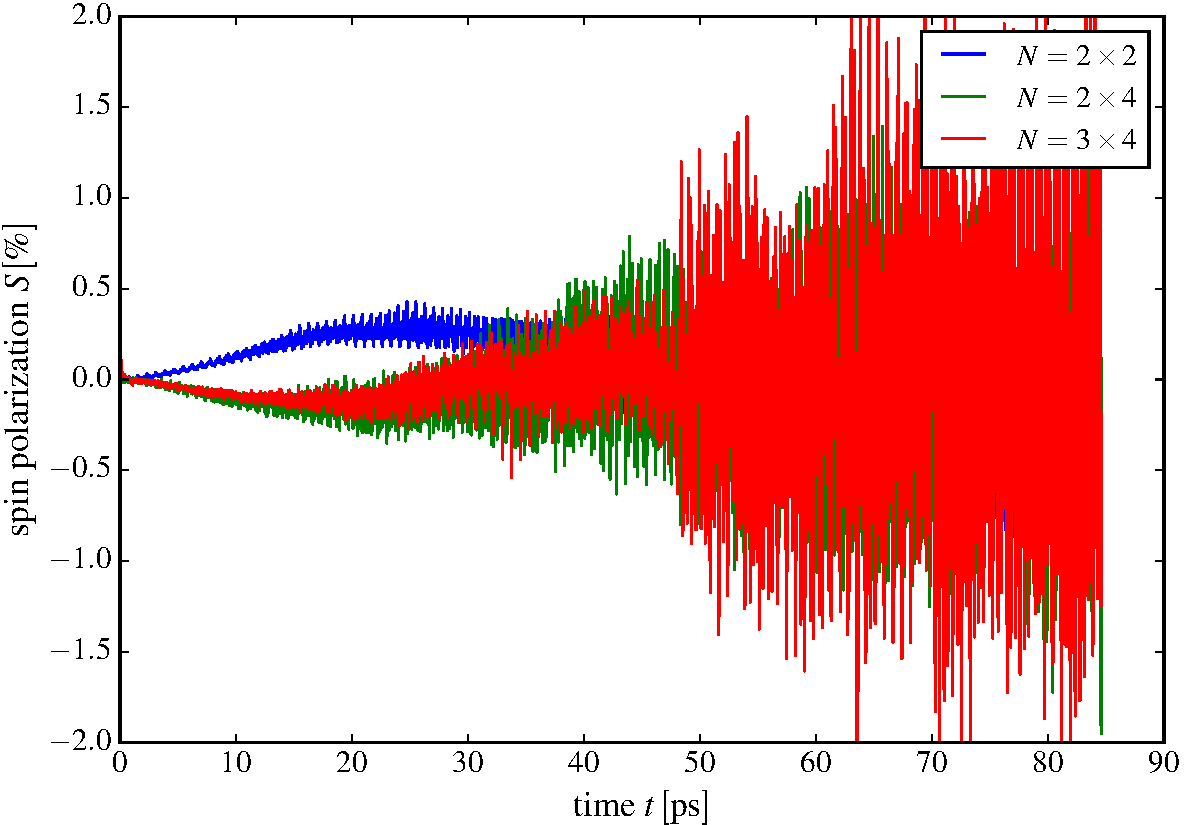
\includegraphics[width=0.45\textwidth]{figs/SpinPolarizations_tsoPh_0.1_N_var_V75.pdf}
	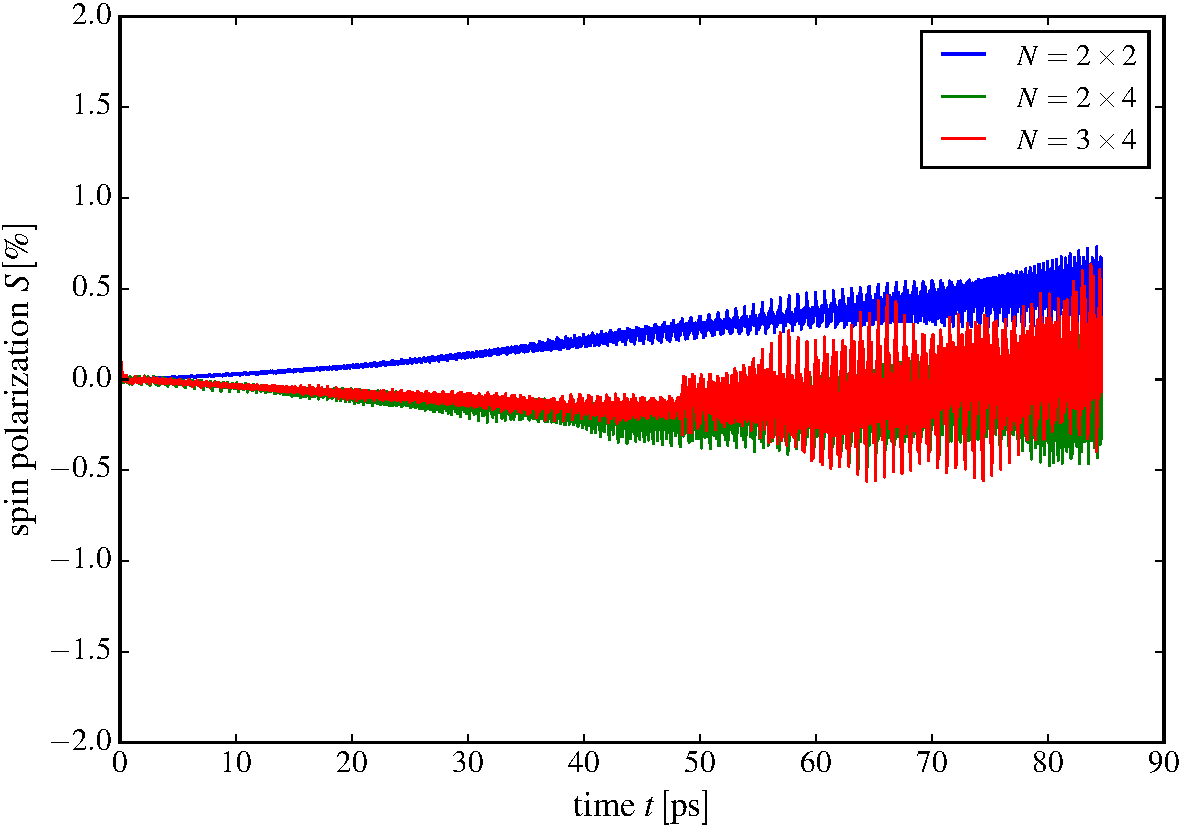
\includegraphics[width=0.45\textwidth]{figs/SpinPolarizations_tsoPh_0.1_N_var_V85.pdf}
	\caption{Comparison of spin polarization for $\lambda_1=\SI{0.1}{\milli\electronvolt}$ and varying system size and $V=\SI{0.6}{\volt}$ (left) and $V=\SI{0.68}{\volt}$ (right).}\label{fig:tsoPh0.1_LVar_2}
\end{figure}
\begin{figure}[!h]
	\centering
	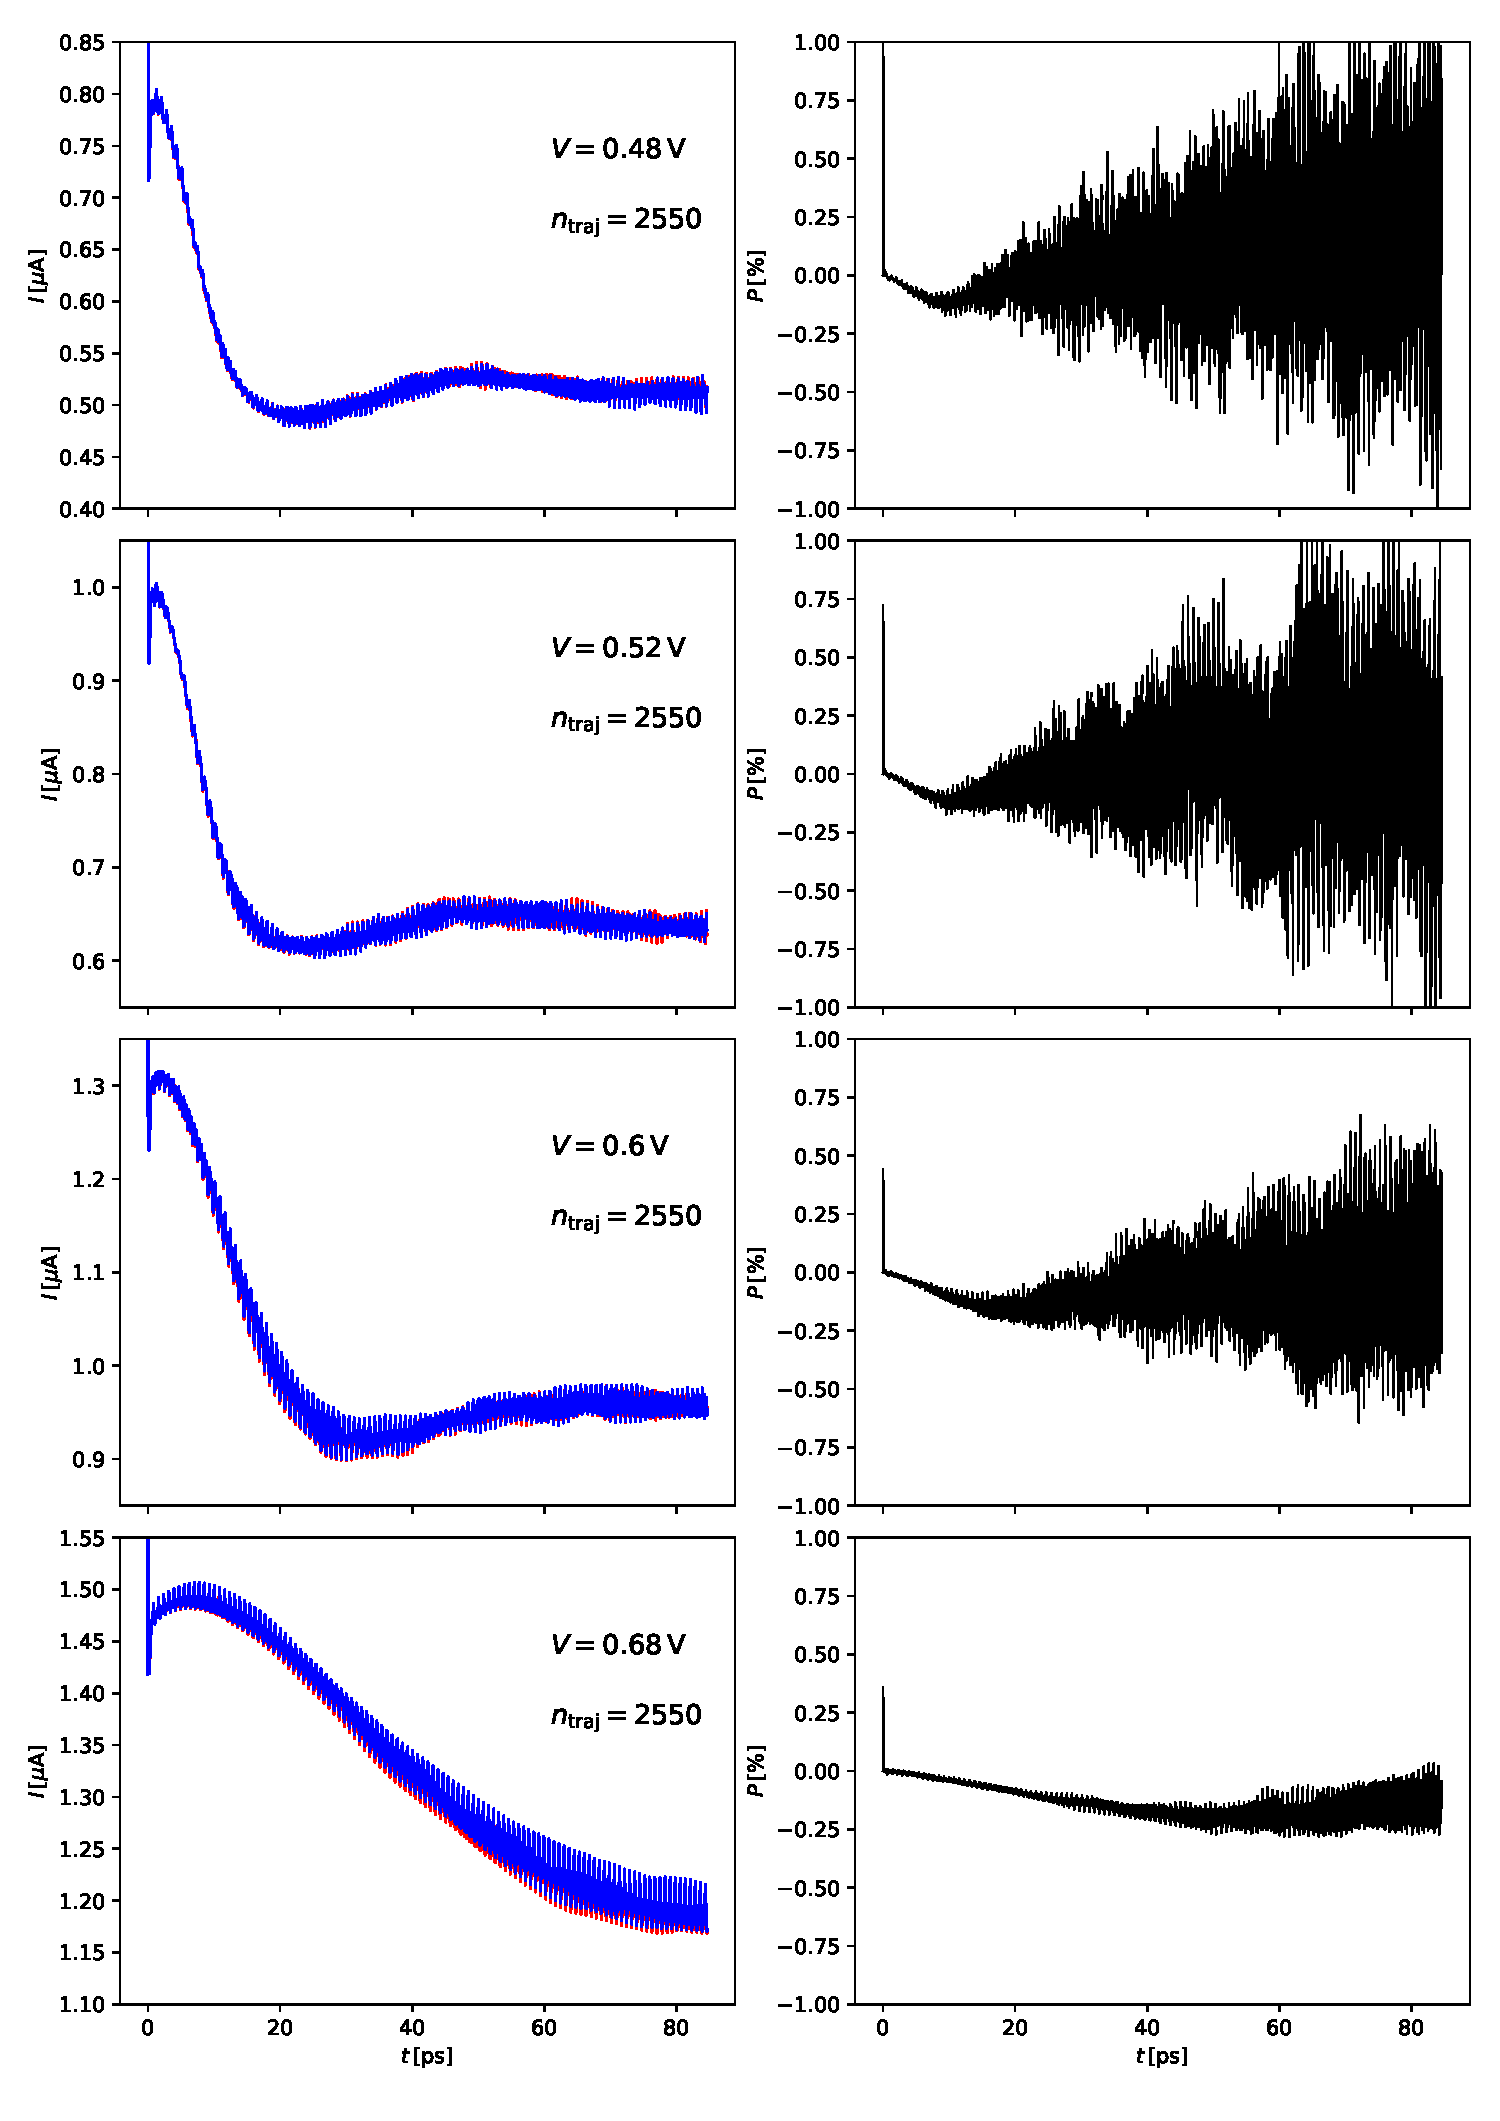
\includegraphics[width=0.9\textwidth]{figs/L2x4_currents_MR_allV_tsoPh0.1.pdf}
	\caption{Charge currents and current polarization for $\lambda_1=\SI{0.1}{\milli\electronvolt}$. Number of trajectories is given in the plot.}\label{fig:L2x4_tsoPh0.1}
\end{figure}
\begin{figure}[!h]
	\centering
	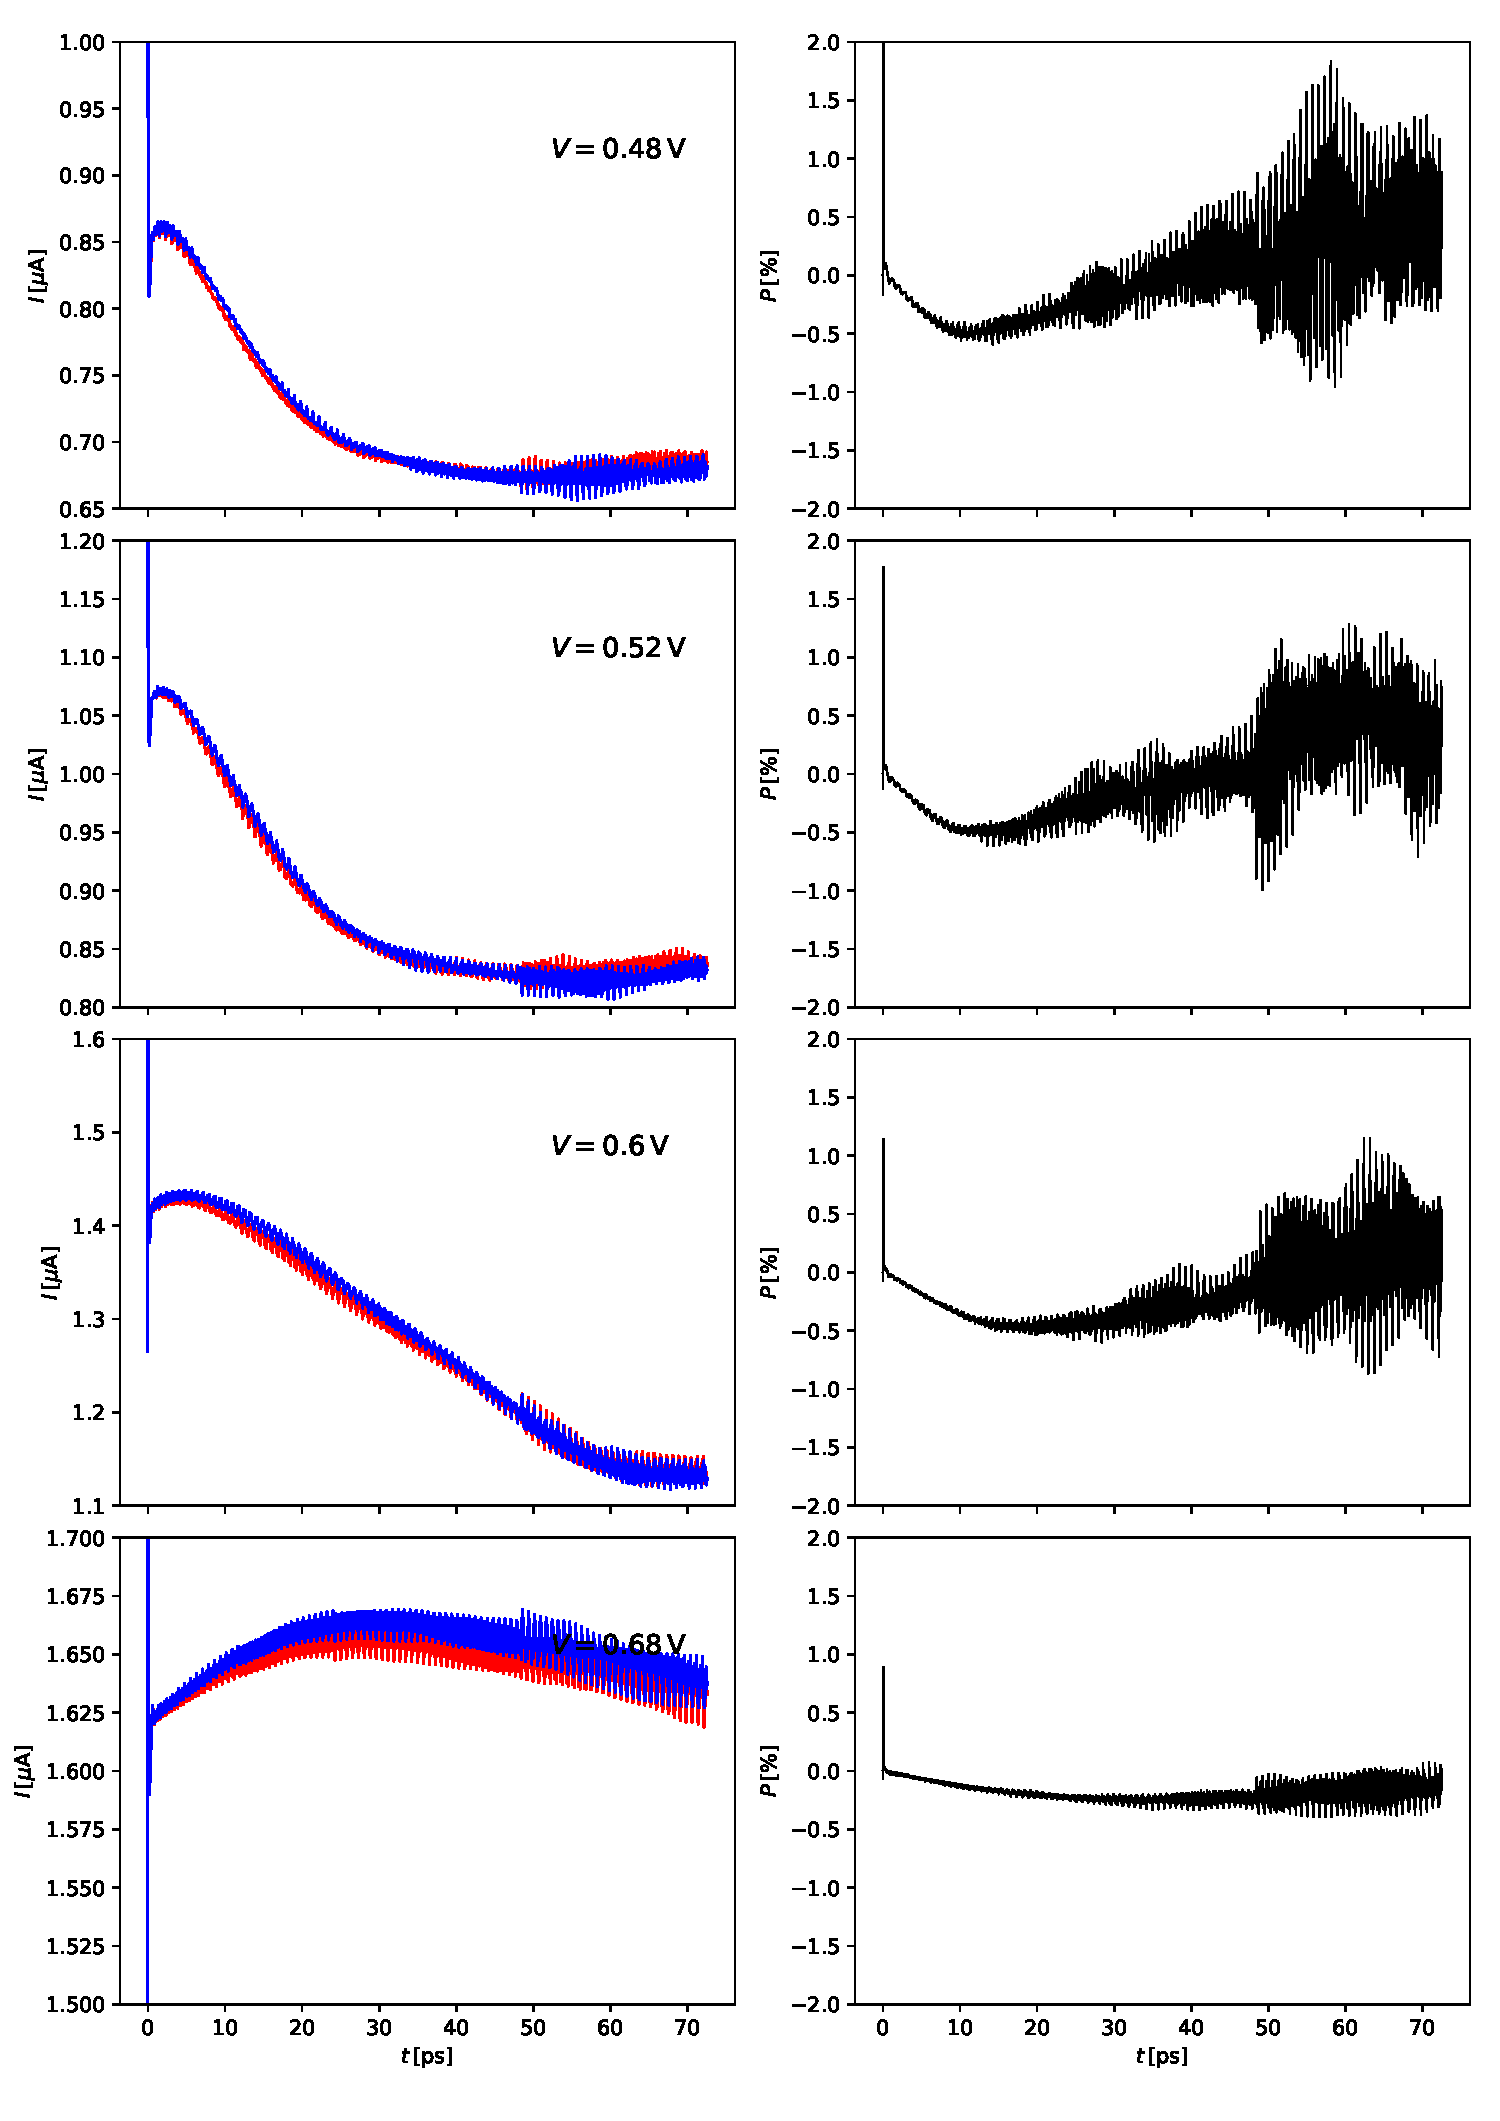
\includegraphics[width=0.9\textwidth]{figs/L2x4_currents_MR_allV_tsoPh5.pdf}
	\caption{Charge currents and current polarization for $\lambda_1=\SI{5}{\milli\electronvolt}$. Data consists of different number of trajectories for different time segments: 20300 for $\SI{0}{\pico\second}\leq t\leq \SI{12}{\pico\second}$, 15200 for $\SI{12}{\pico\second}< t\leq \SI{24}{\pico\second}$ and 11100 for $\SI{24}{\pico\second}< t\leq \SI{48}{\pico\second}$ and 3000 for $t\geq \SI{48}{\pico\second}$ .}\label{fig:L2x4_tsoPh5}
\end{figure}
\begin{figure}[!h]
	\centering
	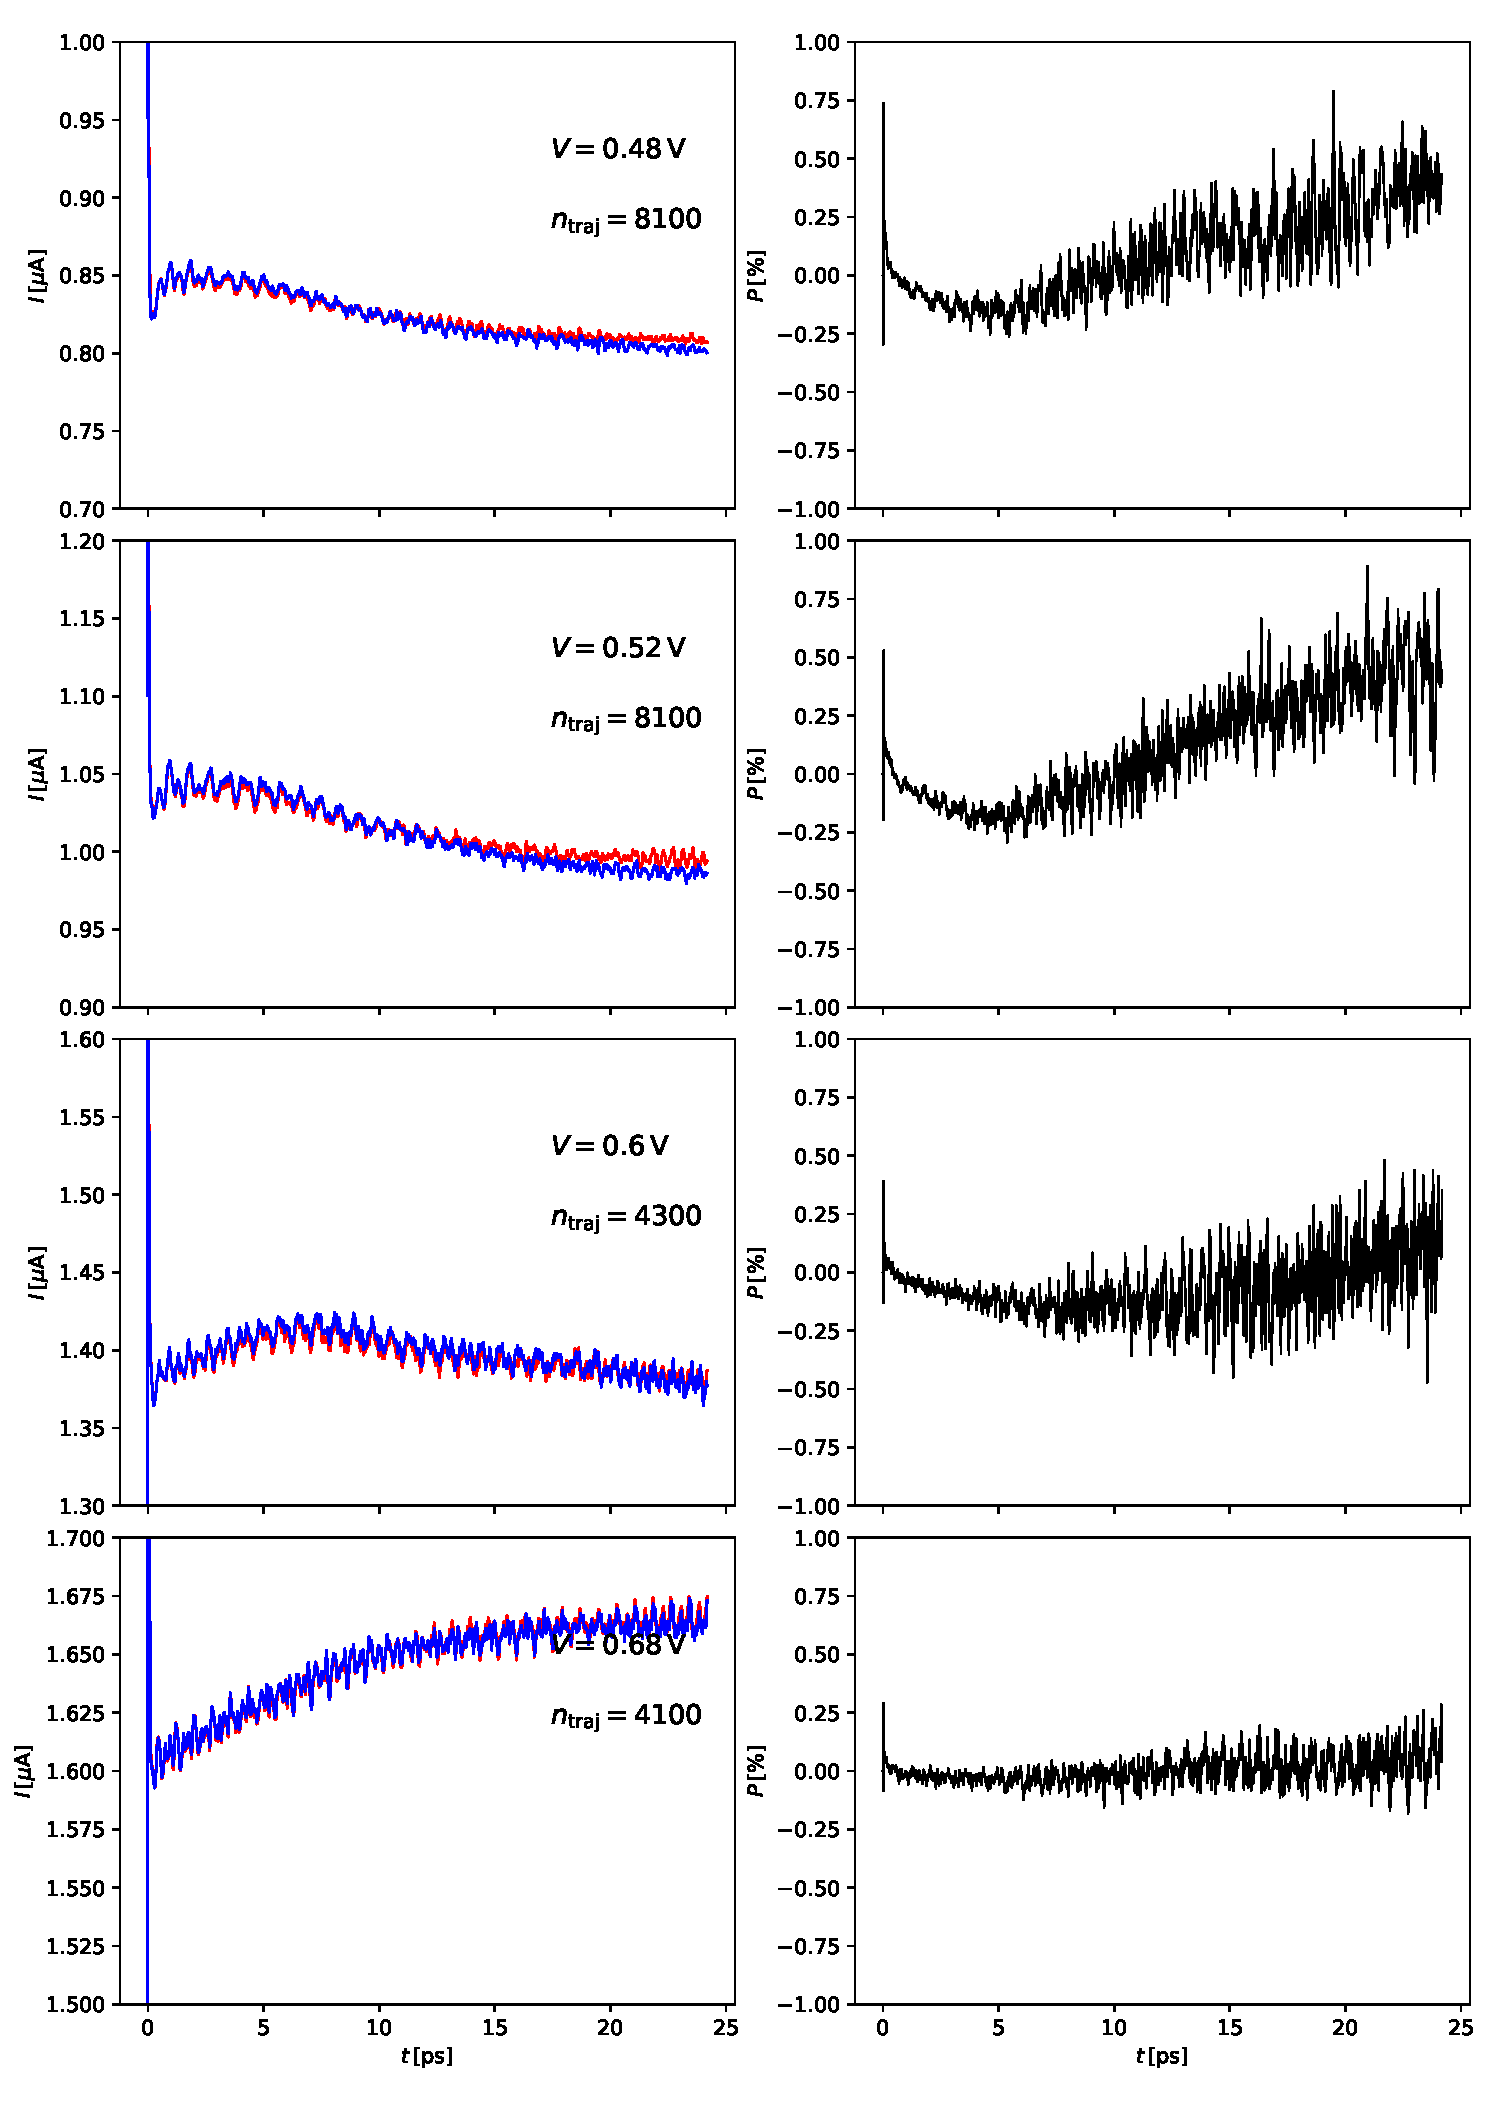
\includegraphics[width=0.9\textwidth]{figs/L2x4_currents_MR_allV_tsoPh10.pdf}
	\caption{Charge currents and current polarization for $\lambda_1=\SI{10}{\milli\electronvolt}$. Data consists of different number of trajectories for different time segments: 26300 for $\SI{0}{\pico\second}\leq t\leq \SI{12}{\pico\second}$, 21200 for $\SI{12}{\pico\second}< t\leq \SI{24}{\pico\second}$ and 13100 for $\SI{24}{\pico\second}< t\leq \SI{48}{\pico\second}$ and 5000 for $t\geq \SI{48}{\pico\second}$ .}\label{fig:L2x4_tsoPh10}
\end{figure}

\begin{figure}[!h]
	\centering
	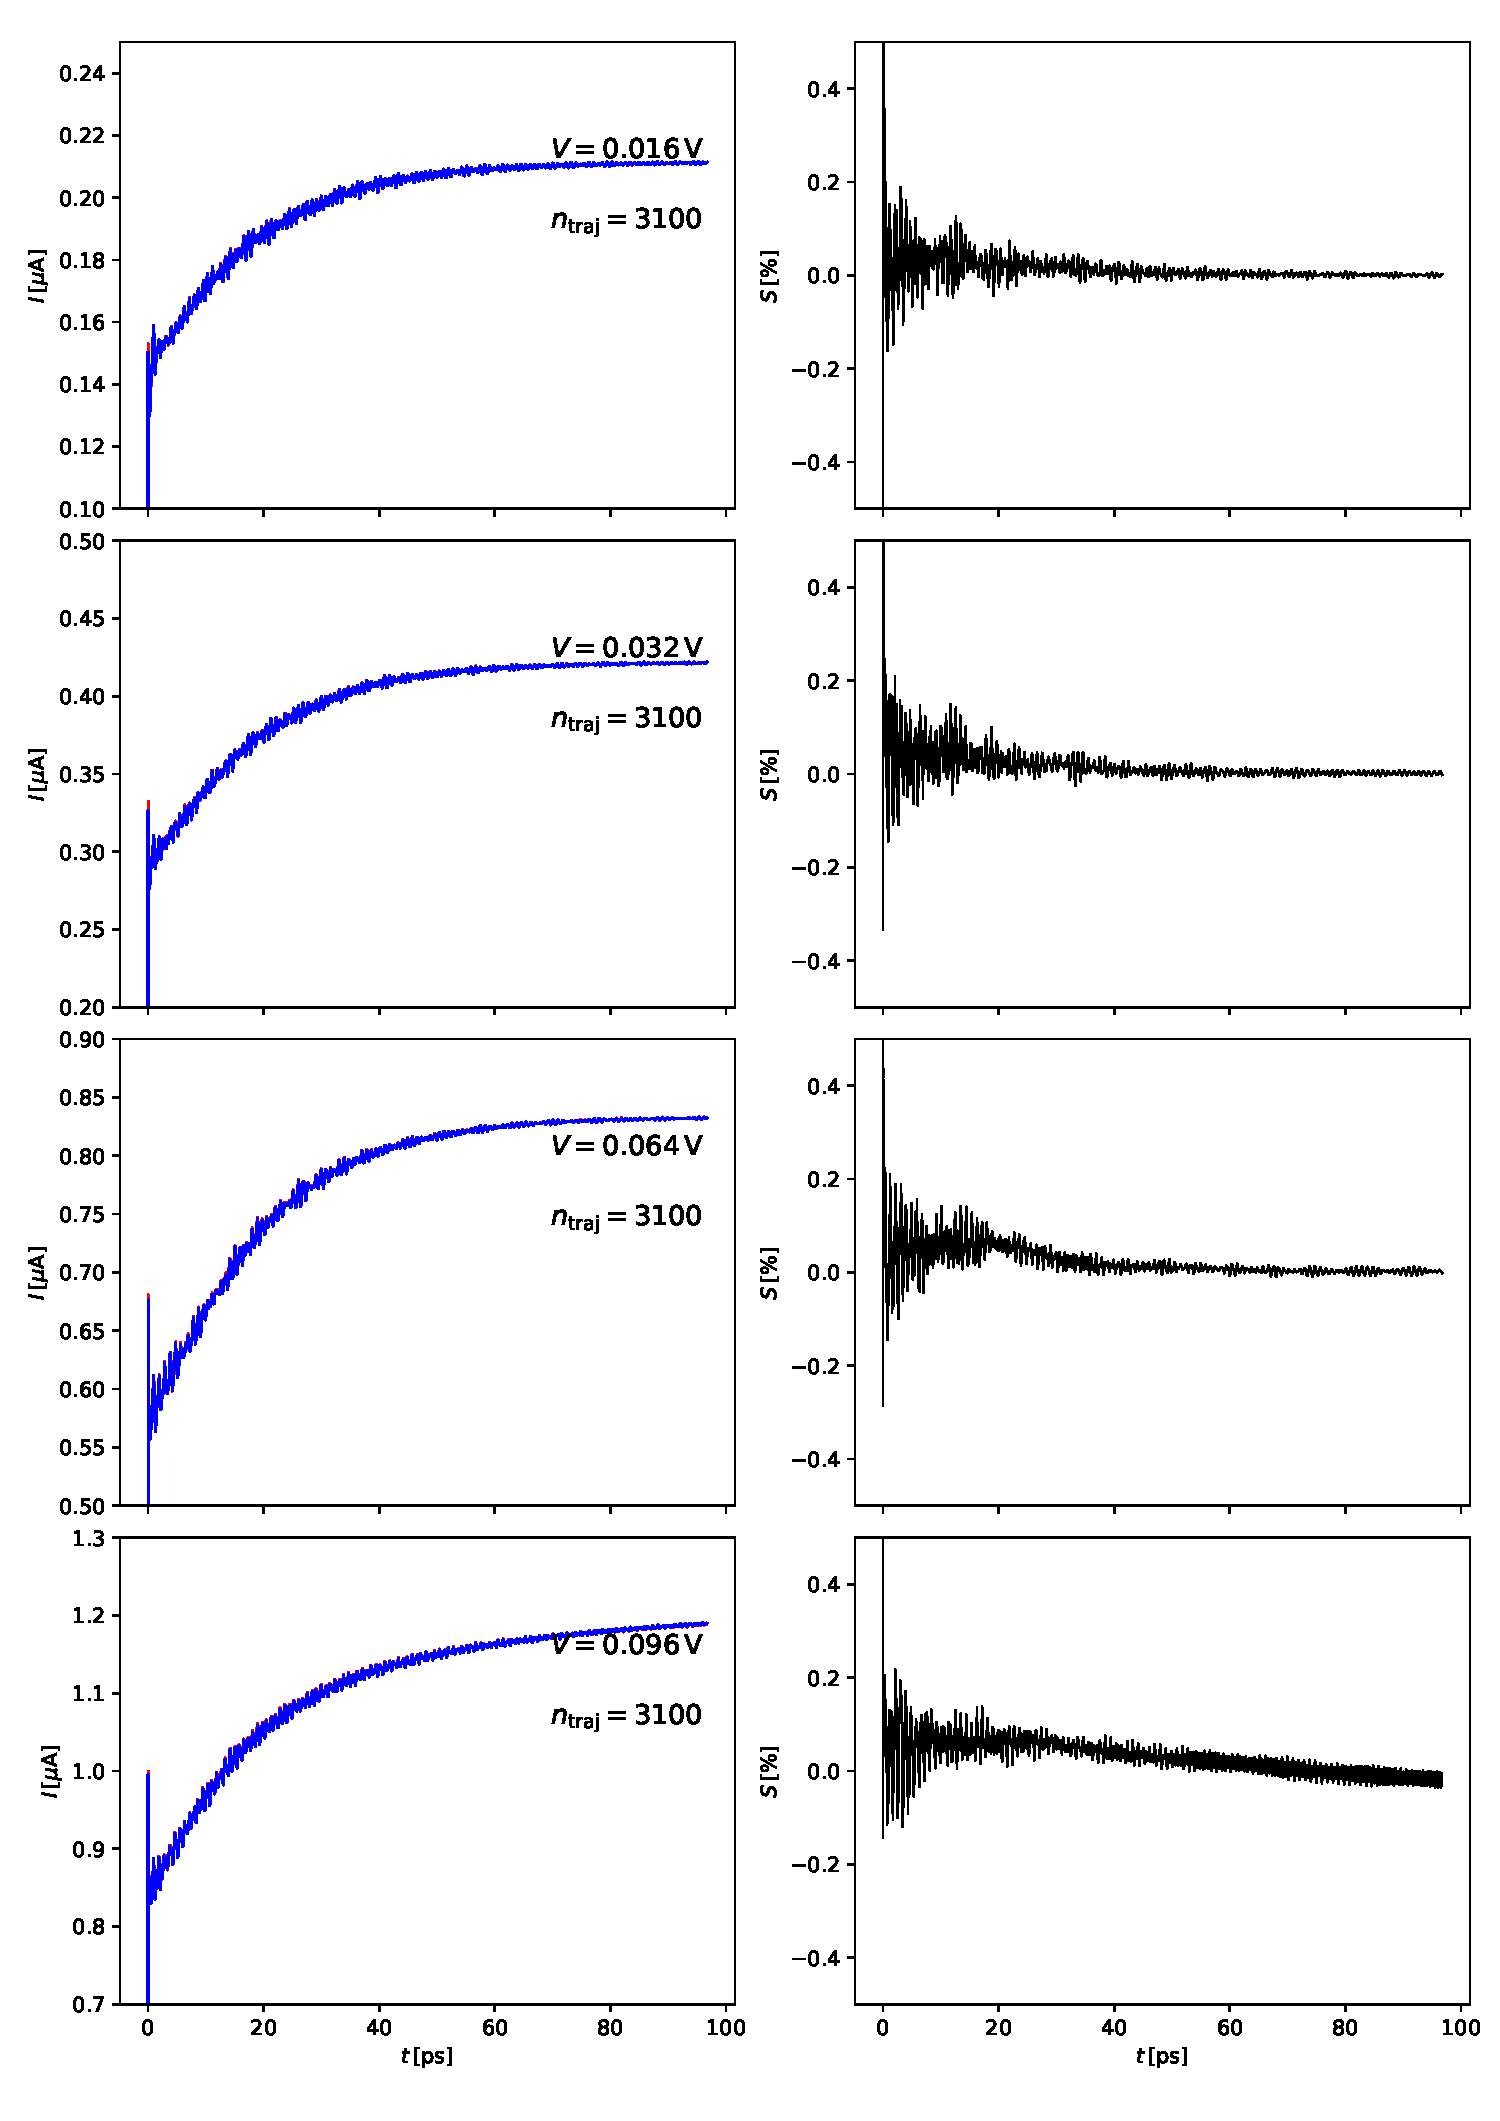
\includegraphics[width=0.9\textwidth]{figs/L2x4_currents_MR_allV_tsoPh10_eps0.pdf}
	\caption{Charge currents and current polarization for $\lambda_1=\SI{10}{\milli\electronvolt}$ and $\varepsilon_0=\SI{0}{\milli\electronvolt}$. Number of trajectories is given in the plot.}\label{fig:L2x4_tsoPh10_eps0}
\end{figure}
\begin{figure}[!h]
	\centering
	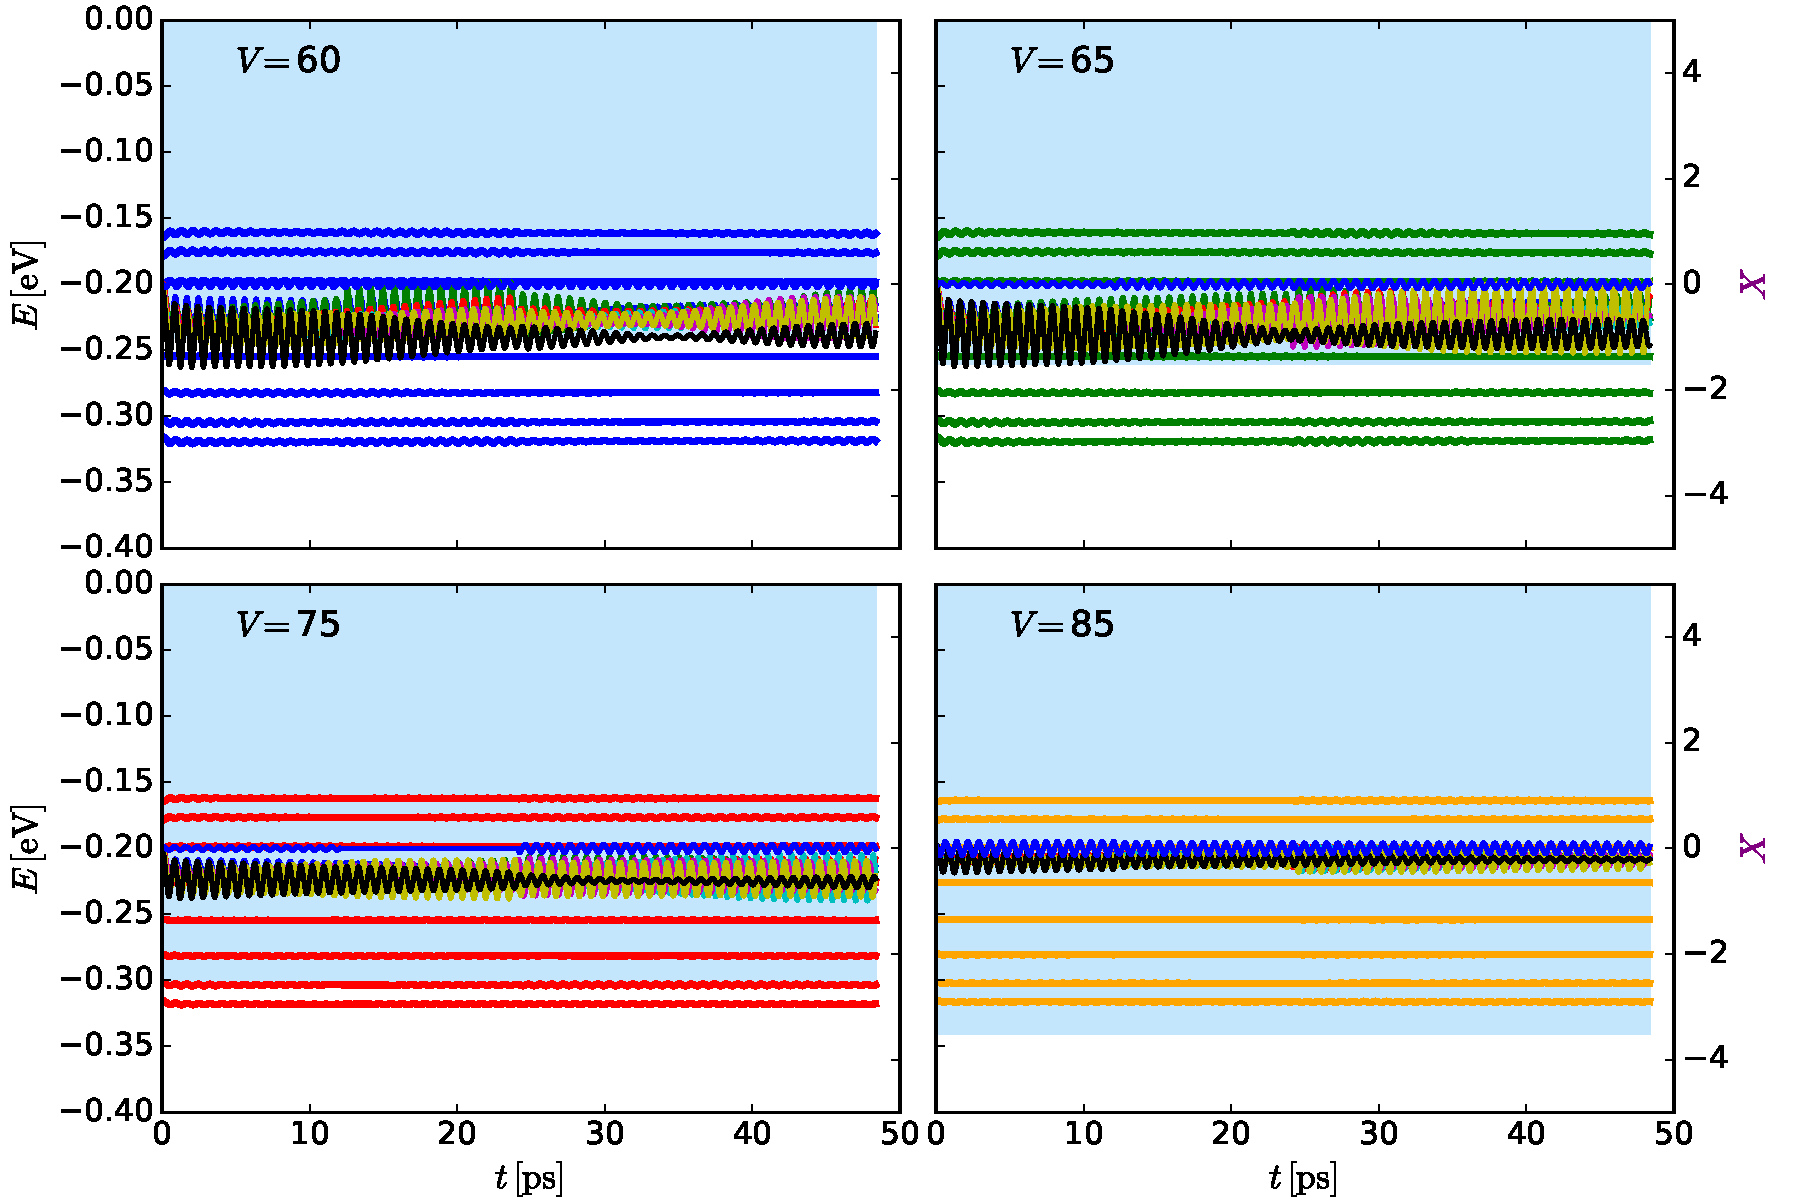
\includegraphics[width=0.9\textwidth]{figs/Fransson_L2x4_tsoPh5.0_spectrum_td_Ph_avg.pdf}
	\caption{Time dependent spectrum under the trajectory-averaged dynamics of the bond displacement for various voltages. Blue area indicates bias window. Same colored lines indicate spectrum, different colored ones the vibrational bond displacement dynamics. SOC-assisted electron-vibrational coupling is $\lambda_1 =\SI{5}{\milli\electronvolt}$.}\label{fig:SpecTD_tsoPh5}
\end{figure}

\begin{figure}[!h]
	\centering
	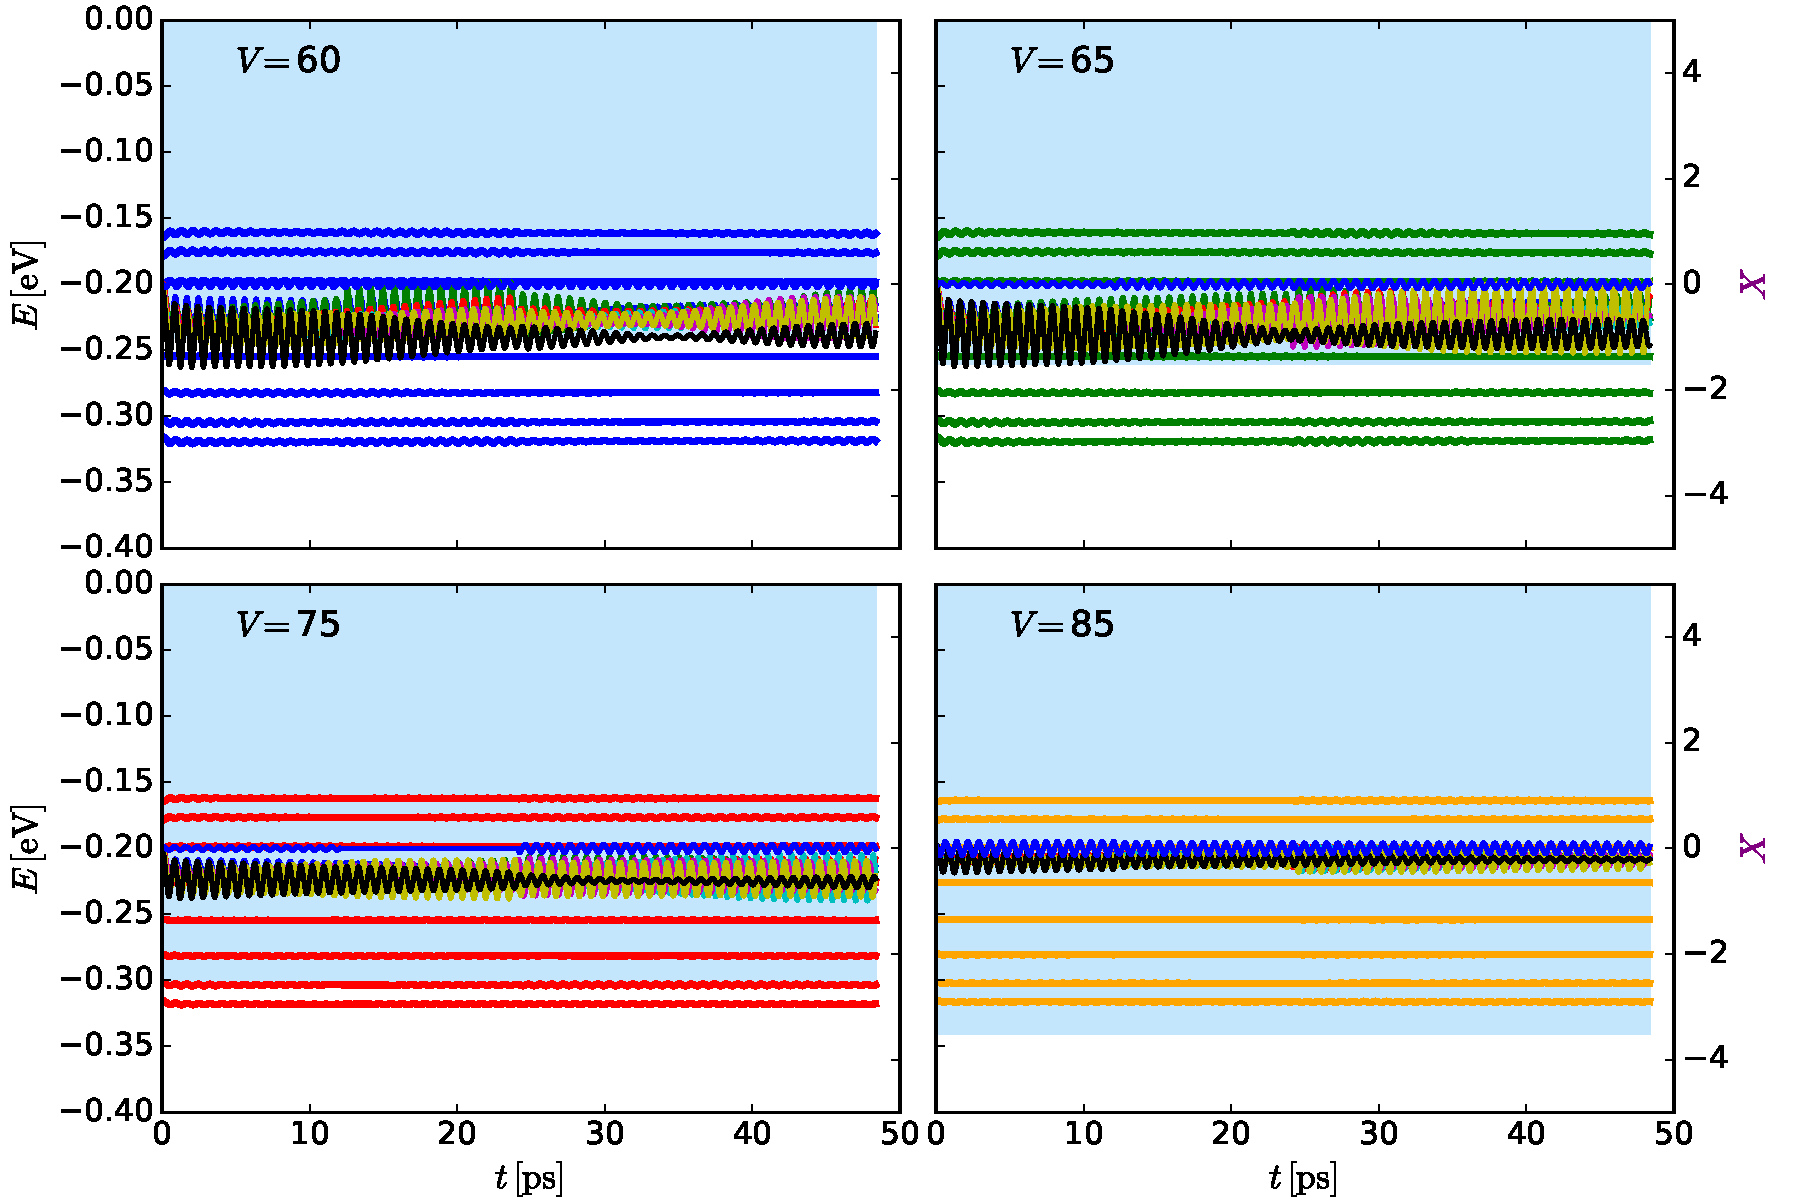
\includegraphics[width=0.9\textwidth]{figs/Fransson_L2x4_tsoPh5.0_spectrum_td_Ph_avg.pdf}
	\caption{Same as in \cref{fig:SpecTD_tsoPh5} for $\lambda_1 =\SI{10}{\milli\electronvolt}$.}\label{fig:SpecTD_tsoPh10}
\end{figure}
\section{Charge current dynamics: TT-HEOM vs Ehrenfest}
\Cref{fig:Comp_TTHEOM_Ehrenfest_t1_4meV} shows the current dynamics obtained from TT-HEOM (blue lines) and from HEOM-Ehrenfest (green lines) and the exact, noninteracting case (red dashed lines) in the Peierls model with three sites. The electron-vibrational coupling is $t_1=\SI{4}{\milli\electronvolt}$ and all other parameters are as in the original problem (except for the SOC, which is set to zero here).
The initial state is an empty molecule in the electronic subspace and the vibrations are in the zero-temperature ground state. For some voltages, the currents obtained from both approaches agree almost quantitatively. However, there are significant differences: For short times, the Ehrenfest approach overestimates charge current oscillations in the off-resonant voltage regime, as can be seen for example for $V=\SI{0.18}{\volt}$ and $V=\SI{0.4}{\volt}$. There, the amplitude of oscillations in the Ehrenfest approach is almost the same as in the noninteracting case. In the TT-HEOM the amplitude of these oscillations is smaller. Therefore, a plausible explanation for this difference is the interaction with the vibrational modes and the different ways it is treated in both approaches. Apart from differences already for short times, there are also differences for long times: While the charge current in the TT-HEOM approaches a steady state already after $\sim \SI{200}{\femto\second}$ (note the time scales of the problem $t_\mathrm{vib}= \omega_0^{-1} \sim \SI{345}{\femto\second}$ and $t_1^{-1}\sim\SI{380}{\femto\second}$). The Ehrenfest approach, however, predicts long-lived charge current oscillations on a much longer time scale than shown in the plot here. These oscillations lead to a deviation from the TT-HEOM result, and for some voltages, e.g., $V=\SI{0.6}{\volt}$, the noninteracting currents agrees with the TT-HEOM one better than the Ehrenfest result. 

{\color{red} Compare Ehrenfest vs TTHEOM for $t_1=\SI{8}{\milli\electronvolt}$. Currently doing convergence checks for TTHEOM.}

\Cref{fig:PES_L1x3} shows the potential energy curve for selected $X_2$ positions. One can see for certain vibrational positions nearly crossing potential energy surfaces. The interesting thing is that for very large displacement, the potential energy surface corresponding to the lowest state is near flat. Therefore, the mean potential energy will also not be bounded if only the lowest electronic state is populated.
\begin{figure}[!h]
	\centering
	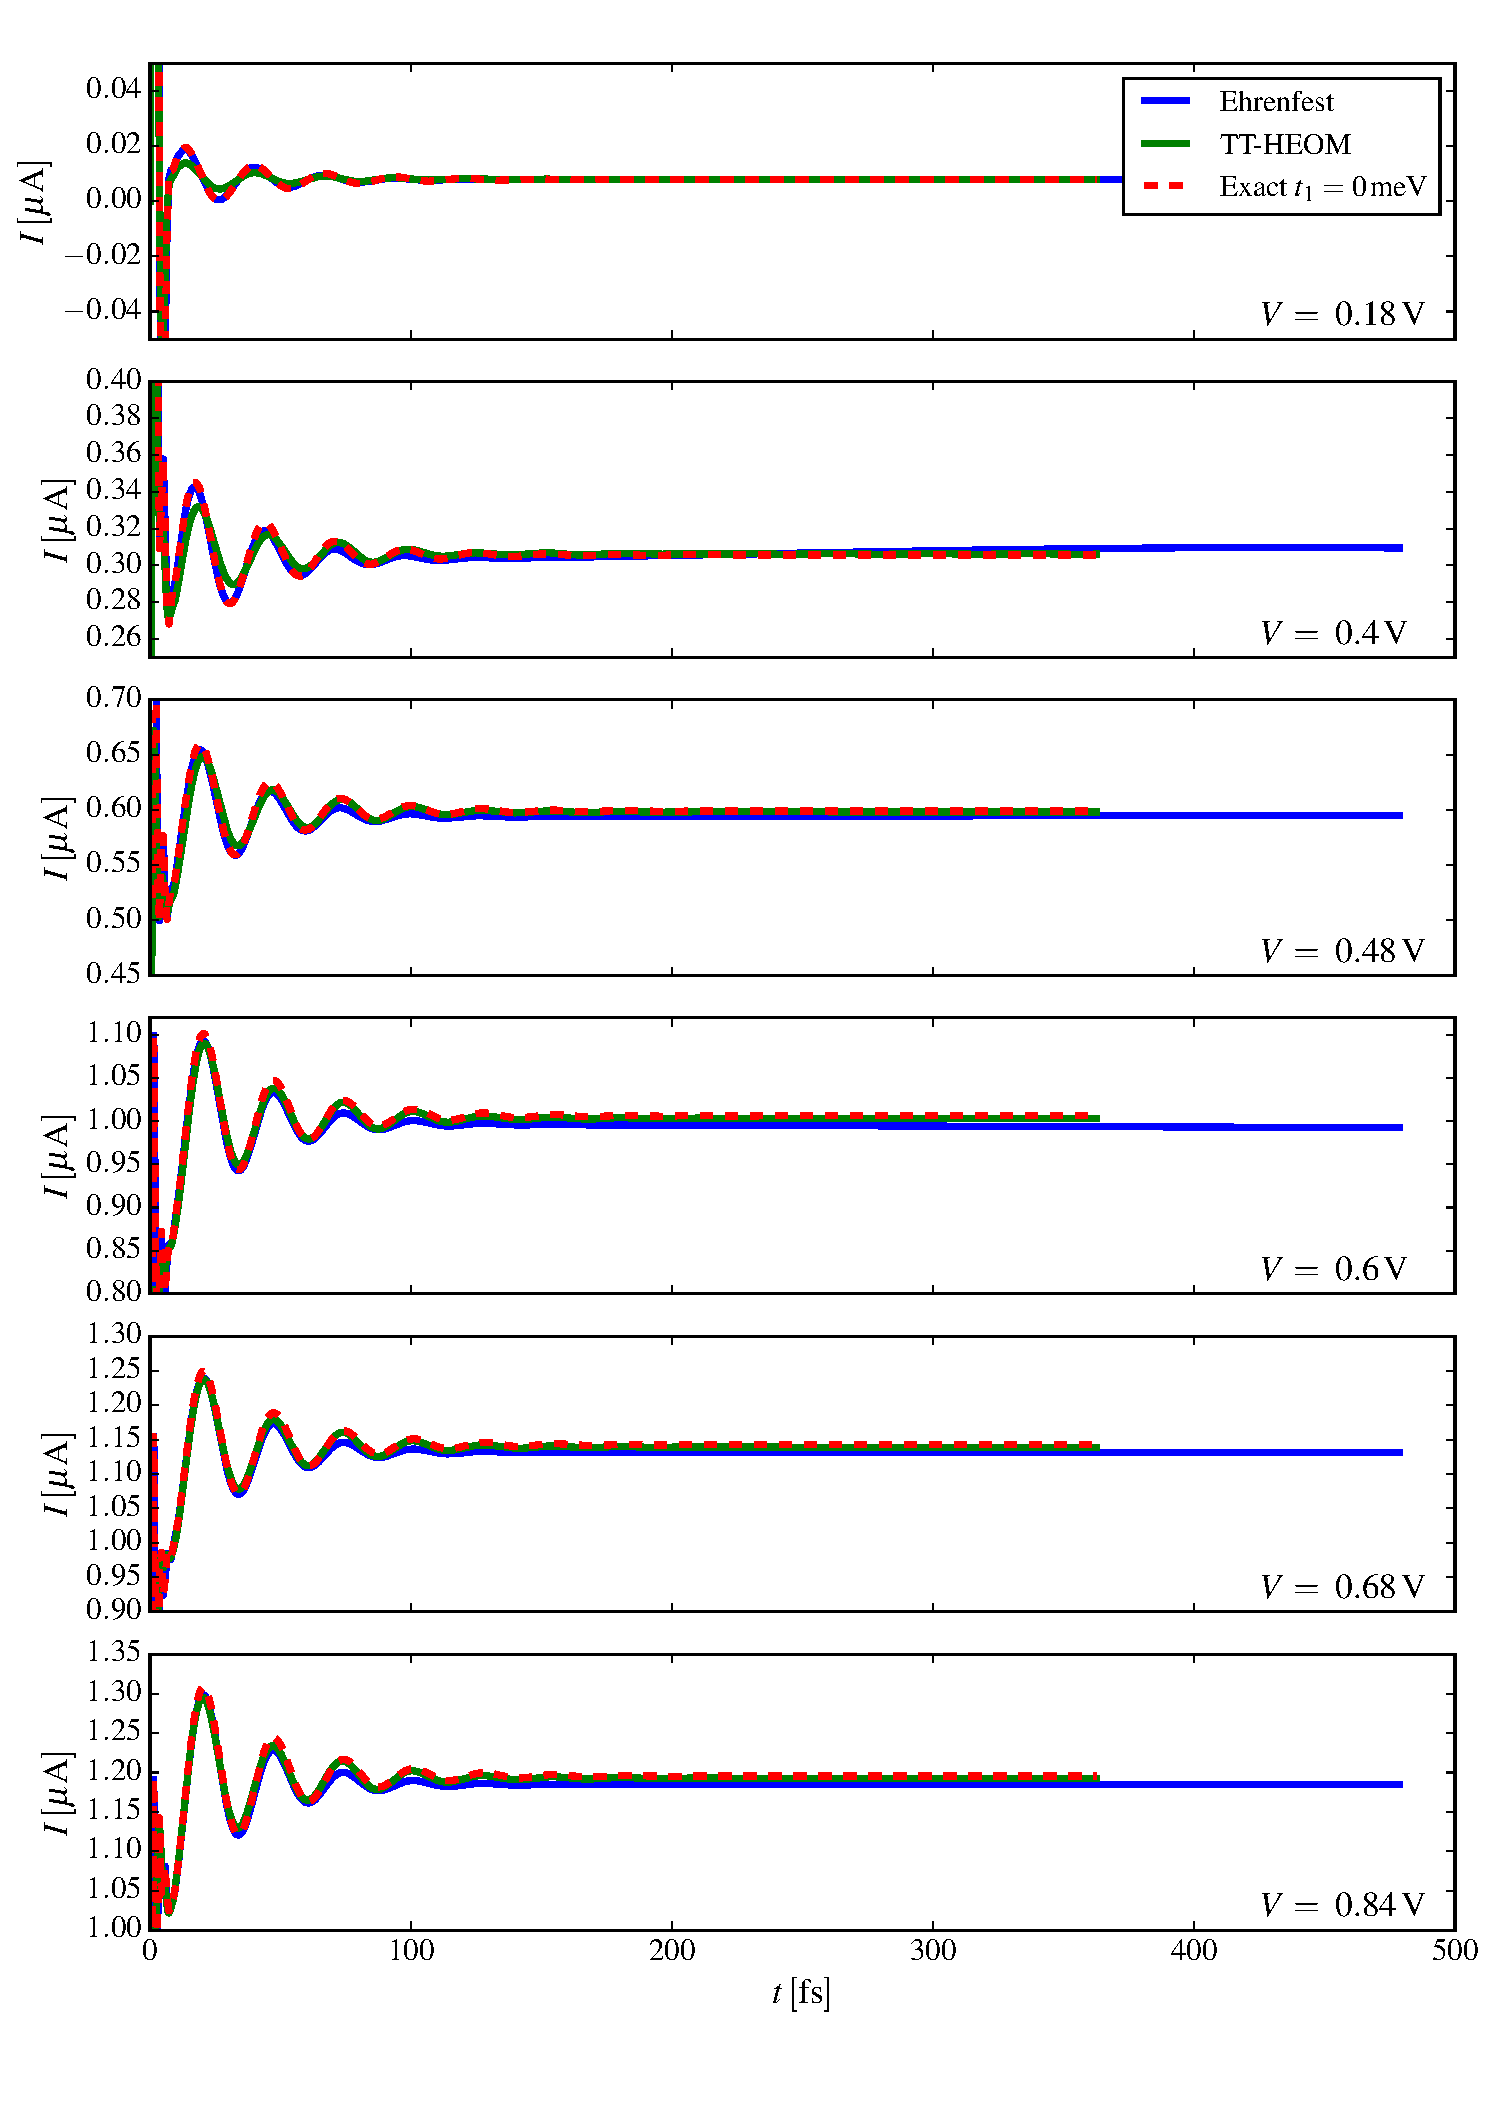
\includegraphics[width=0.9\textwidth]{figs/Peierls_dyn_TTHEOM_Ehrenfest_noPh_VVar.pdf}
	\caption{Charge current dynamics in the three-site spinless Peierls model with $t_1=\SI{4}{\milli\electronvolt}$: Ehrenfest (blue), TT-HEOM (green) and the exact, noninteracting case (red dashed line).}\label{fig:Comp_TTHEOM_Ehrenfest_t1_4meV}
\end{figure}
\begin{figure}[!h]
	\centering
	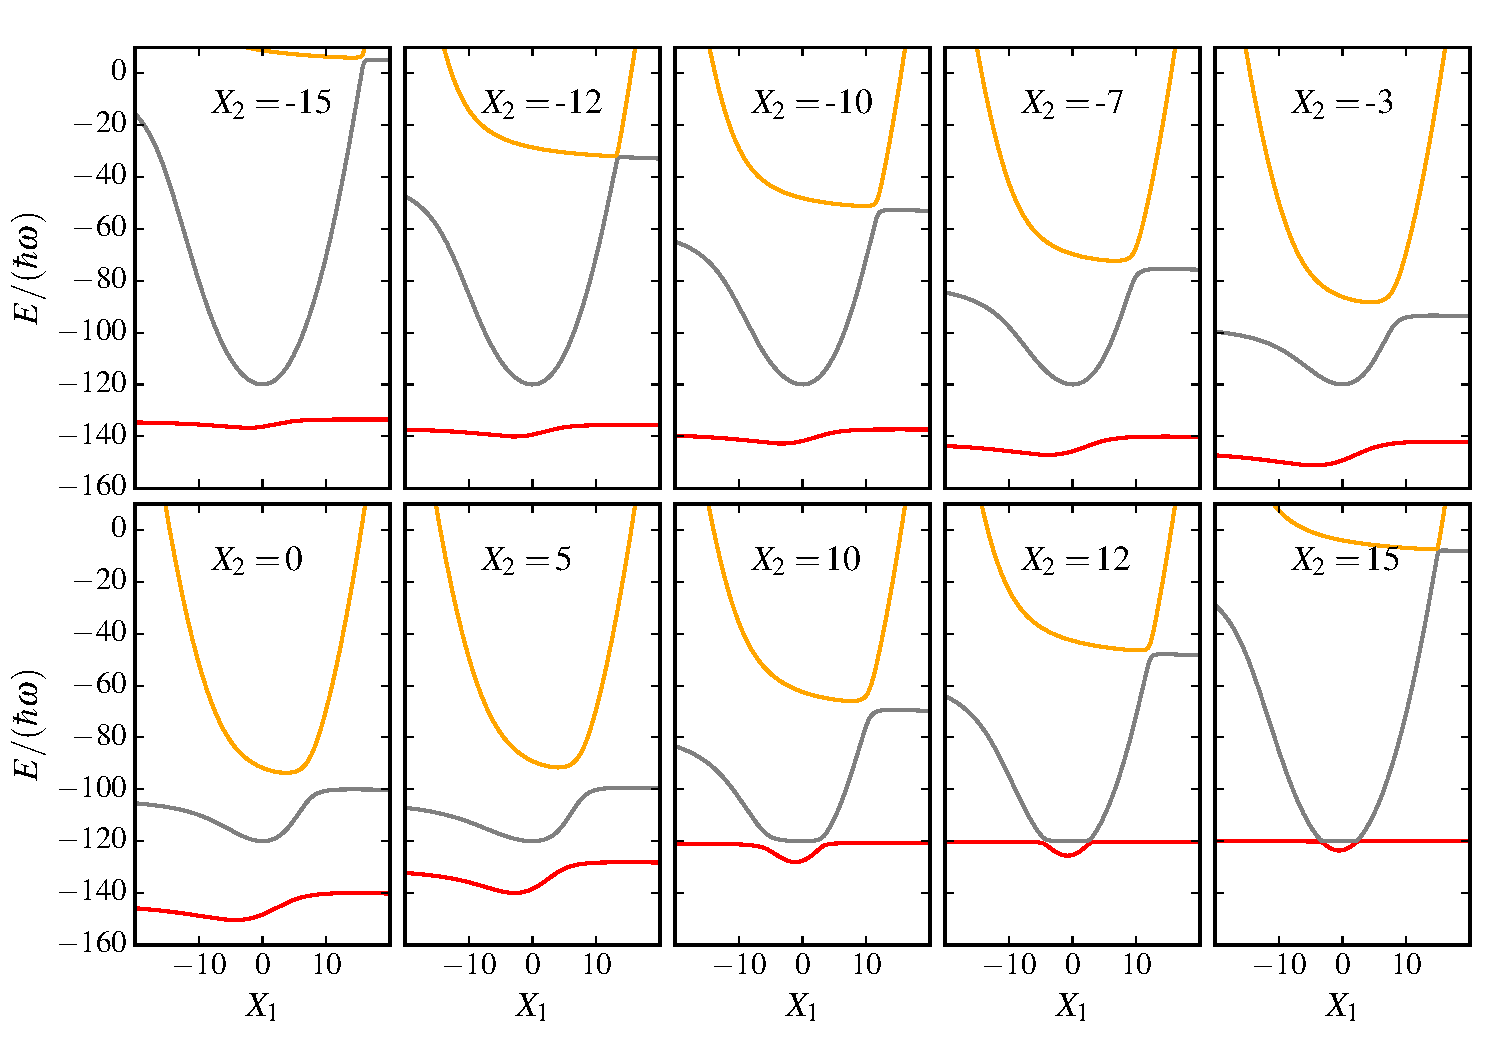
\includegraphics[width=1\textwidth]{figs/PES_1x3_SOC0.0_tPh2.0_SOCPh0.0_multiState_cuts_v2.pdf}
	\caption{Potential energy curves for the model investigated in \cref{fig:Comp_TTHEOM_Ehrenfest_t1_4meV}.}\label{fig:PES_L1x3}
\end{figure}
\clearpage
\section{Fixed point analysis of the classical Peierls model}
{\color{red} Do the same analysis as in \cite{sakkinen2015many} for the two-site one mode and three-sites two-modes Peierls model. Try to do this also for the open system using HEOM.}
\subsection{Two-site, one mode model}
The two-site Peierls model within the Ehrenfest approximation consists of the quantum Hamiltonian
\begin{equation}
	H_q(t) = H_\mathrm{el} + H_\mathrm{el-vib}(t) =  \left(-t_0+t_1 X(t)\right)(c_1^\dagger c_2^\pdagger+ \mathrm{h.c.}) 
\end{equation}
and the classical Hamiltonian
\begin{equation}
	H_c(t) = \frac{1}{2}\left(X^2 + P^2\right) + \tr{\rho(t)H_\mathrm{el-vib}}.
\end{equation}
\subsubsection{Isolated system}
The Ehrenfest equations of motion read 
\begin{align}
	\dot{\rho} &= -i[H_q,\rho] = 
	-i(-t_0+t_1X)\begin{pmatrix}
		c^*-c & 1-2n\\
		2n-1 & c-c^*
	\end{pmatrix}
	\label{eq:QEOM_P2}\\
	\dot{X} &= P \label{eq:HEOM_P2_1}\\
	\dot{P} &= -X - \tr{\rho\partial_X H_\mathrm{el-vib}} = -(X+t_1(c+c^*)) \label{eq:HEOM_P2_2}
\end{align}
where we $c$ is the off-diagonal element in $\rho$ and $n$ is the occupation of first site. The occupation of the second site can be obtained from $n_2 = 1-n$.
Solving for the equilibrium fixed point, one obtains the following set of conditions
\begin{eqnarray}
	\mathrm{(i)} &  i(t_0-t_1X) \begin{pmatrix}
		c^*-c & 1-2n\\
		2n-1 & c-c^*
	\end{pmatrix} & = 0\\
	\mathrm{(ii)} & P &= 0\\
	\mathrm{(iii)} & X + t_1(c+c^*) &= 0\\
	\overset{\mathrm{(iii)}}{\Rightarrow} &X&= -t_1(c+c^*)\\ \overset{\mathrm{(i)}}{\Rightarrow} &  X &= \frac{t_0}{t_1} \qquad \mathrm{(a)} \\
	& \vee  \begin{pmatrix}
		c^*-c & 1-2n\\
		2n-1 & c-c^*
	\end{pmatrix} & = 0 \Rightarrow n=\frac{1}{2}, c^*=c \qquad \mathrm{(b)}.
\end{eqnarray}
For $X=\frac{t_0}{t_1}$ there exist a family of fixed points given by
\begin{equation}
	\xi_1 = \left(n=\frac{1-m}{2}, c = -\frac{1}{2}\left(\frac{t_0}{t_1^2}+k\right), X=\frac{t_0}{t_1}, P = 0 \right),\qquad k\in\mathds{C}, 0<m\leq 1,
\end{equation}
determined by two parameters $k$ and $m$, which are fixed by the initial condition.
In the other case there exists also a family of fixed points
\begin{equation}
	\xi_2 = (n = \frac{1}{2}, c=c, X=-2t_1c , P=0), \qquad c\in\mathds{R},
\end{equation}
which is, however, determined by a single parameter $c$. Below we will give conditions on these free parameters following from energy conservation.
Note that the coherence has to be real in the case (b) because we assume that the displacement of the classical mode is real as well.
Both fixed points are subject to the constraint that the total energy is conserved, which is in the Ehrenfest approach the sum of the energies of both subsystems
\begin{align}
	E &= E_q + E_c  \\
	 &= \langle H_q\rangle + H_c\\
	 &= (-t_0+t_1 X)(c+c^*) + \frac{1}{2}(X^2+P^2).\\
\end{align}
At both fixed points $P=0$, and hence this part can be neglected in the energy.
The first fixed point leads to the following total energy
\begin{equation}
	E_1 = \frac{1}{2}\left(\frac{t_0}{t_1}\right) \Rightarrow X = \pm\sqrt{2E_1} , c=-\frac{1}{2}\left(\frac{\pm\sqrt{2E_1}}{t_1}+k\right).  
\end{equation}
The first fixed point consists of infinitely many fixed point, defined by all possible initial conditions, and thus $k$. 
For the second fixed point one obtains the following energy
\begin{equation}
	E_2 = -2t_0c - 2t_1^2 c^2,
\end{equation}
which determines $c$ 
\begin{align}
	c_{2\pm} &= -\frac{t_0}{2t_1} \pm\sqrt{\left(\frac{t_0}{2t_1}\right)^2 - \frac{E_2}{2t_1}}.
\end{align}
Thus, the second fixed point consists only of two fixed points, namely depending on whether the coherence is the $+$ or $-$ solution given above. 
The next step is to analyze the stability of these fixed points. This is achieved by analyzing the eigenvalues of the Jacobian of the system 
\begin{align}
	\mathds{J} = \begin{pmatrix}
		\partial_n f & \partial_c f & \partial_X f & \partial_P f\\
		\partial_n g & \partial_c g & \partial_X g & \partial_P g
	\end{pmatrix}
\end{align}  
where $f$ and $g$ are the right-hand-sides of the quantum and classical equations of motion, respectively, given in \cref{eq:QEOM_P2,eq:HEOM_P2_1,eq:HEOM_P2_2} (for the quantum equations of motion we only consider the parts corresponding to $\dot{n}$ and $\dot{c}$).
The Jacobian is 
\begin{equation}
	\mathds{J} =\begin{pmatrix}
		\begin{pmatrix}
			0 \\ -2i(t_0-t_1X)
		\end{pmatrix} & 
		\begin{pmatrix}
			-i(t_0-t_1X) \\ 0
		\end{pmatrix} &
		\begin{pmatrix}
			-it_1 (c^*-c) \\ -it_1(1-2n)
		\end{pmatrix} &
		\begin{pmatrix}
			0 \\ 0
		\end{pmatrix}
\\
\begin{pmatrix}
	0 \\ 0
\end{pmatrix} & \begin{pmatrix}
0 \\ -t_1
\end{pmatrix}
& \begin{pmatrix}
	0 \\ -1
\end{pmatrix}
& \begin{pmatrix}
	1 \\ 0
\end{pmatrix}
	\end{pmatrix}.
\end{equation}
At the first family of fixed points, the Jacobian is
\begin{equation}
	\mathds{J}_1 =\begin{pmatrix}
		0 & 0 & it_1k & 0\\
		0 & 0 & -it_1 m & 0\\
		0 & 0 & 0 & 1 \\
		0 & -t_1 & -1 & 0
	\end{pmatrix}
\end{equation}
with $k=2\mathrm{Im}(c)$. Has a pitchfork-bifurcation for varying filling $n$ at $t_1=\frac{\SI{4}{\milli\electronvolt}}{\hbar \omega}$. 
\Cref{fig:J1_mVar_c1_0.0,fig:J1_mVar_c1_0.1,fig:J1_cVar_m0,fig:J1_cVar_m0.5} show the real and imaginary parts of the eigenvalues of the Jacobian $\mathbb{J}_1$ for varying fillings and coherences.  
The spectrum of $\mathbb{J}_1$ contains local bifurcations, that is changes in the character of the equilibrium points, both in real and imaginary eigenvalues as the filling $n$ is changed. 
The real part of the eigenvalues of $\mathbb{J}_1$ has a pitchfork bifurcation of the fixed points at $n=\frac{1}{2}\pm \frac{19}{400}$. The imaginary part has three bifurcation points for varying $n$. One at $n=\frac{1}{2}$ and another two at $n=\frac{1}{2}\pm \frac{1}{20}$.
The latter two points mark the fillings at which the spectrum of $\mathbb{J}_1$ is the complex conjugate one of the spectrum at fillings mirrored at half-filling. For all fillings except $n=\frac{1}{2}$ at which the equilibrium point is a unstable saddle point, the eigenvalues are complex with unequal signs and some have a positive real part. Hence, the equilibrium point $\xi_1$ is not asymptotically stable. It rather resembles the structure of a strange attractor. 
The coherence does not affect the spectrum much, as can be seen in comparing \cref{fig:J1_mVar_c1_0.0} with   \cref{fig:J1_mVar_c1_0.1} which shows the spectrum for $c=0$ and $c=0.1+0.01i$, respectively, or in \cref{fig:J1_cVar_m0,fig:J1_cVar_m0.5}.
\begin{figure}[!h]
	\centering
	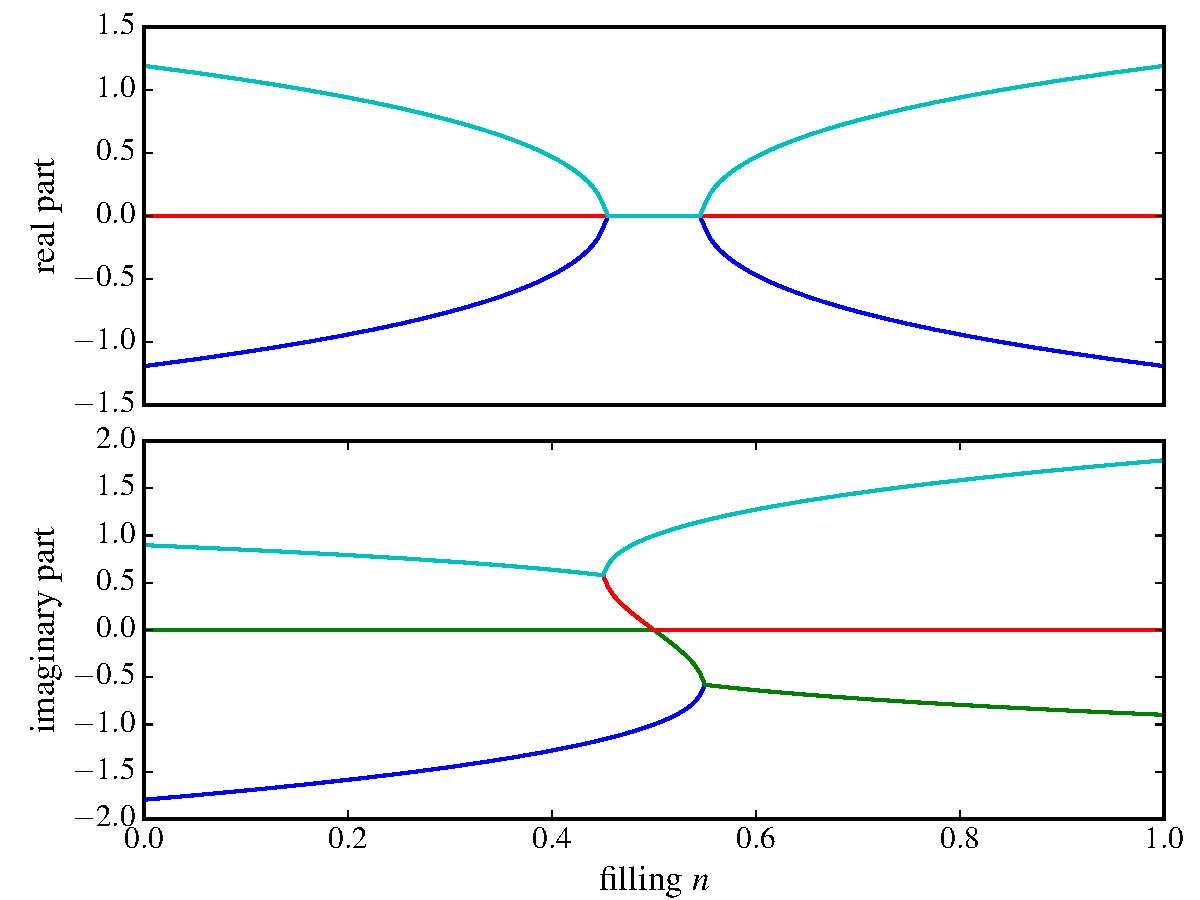
\includegraphics[width=0.7\textwidth]{figs/J1_eigenvalues_mVar_t1_0.004_c1_0.0.pdf}
	\caption{Variation of real and imaginary part of eigenvalues of $\mathbb{J}_1$ for varying filling $n$ for $c=0$.}\label{fig:J1_mVar_c1_0.0}
\end{figure}
\begin{figure}[!h]
	\centering
	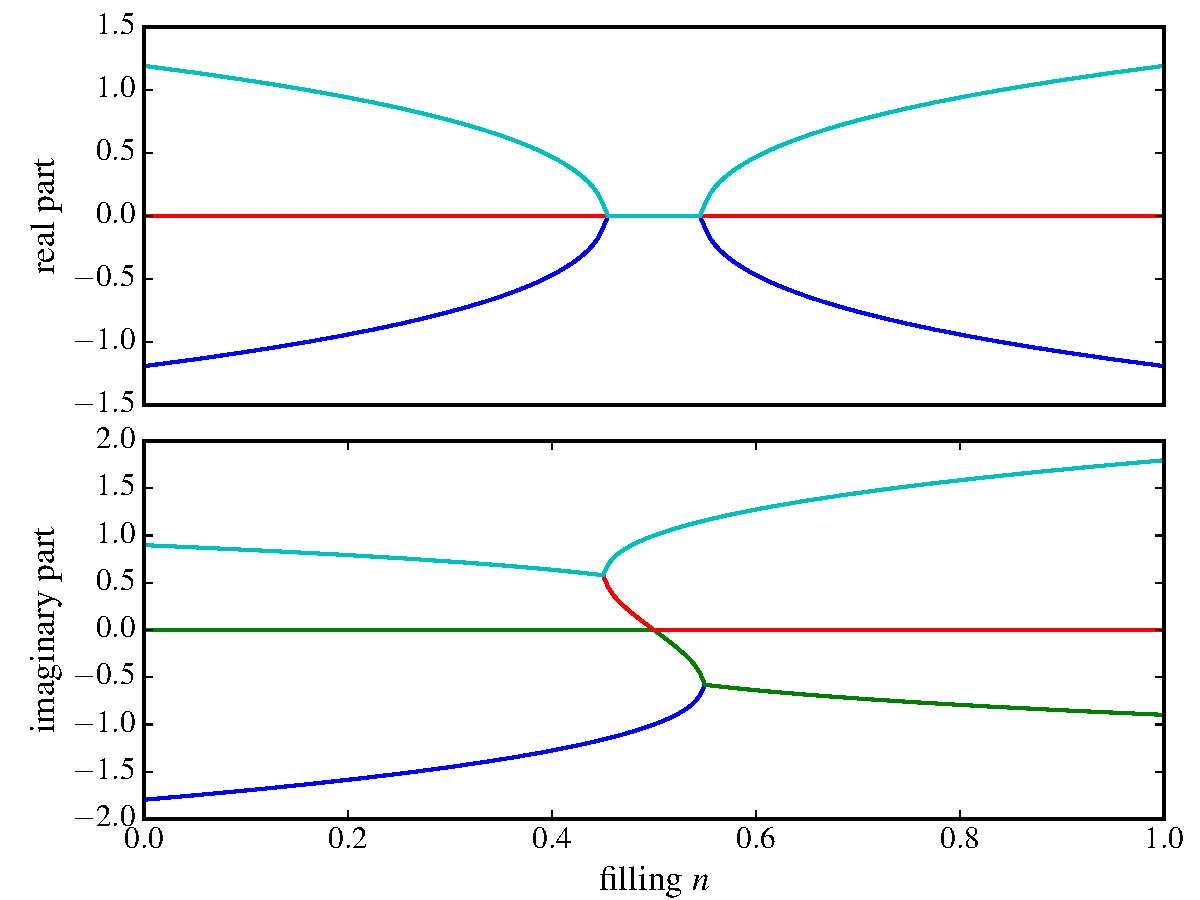
\includegraphics[width=0.7\textwidth]{figs/J1_eigenvalues_mVar_t1_0.004_c1_0.1004987562112089.pdf}
	\caption{Variation of real and imaginary part of eigenvalues of $\mathbb{J}_1$ for varying filling $n$ for $c=0.1+0.01i$.}\label{fig:J1_mVar_c1_0.1}
\end{figure}

\begin{figure}[!h]
	\centering
	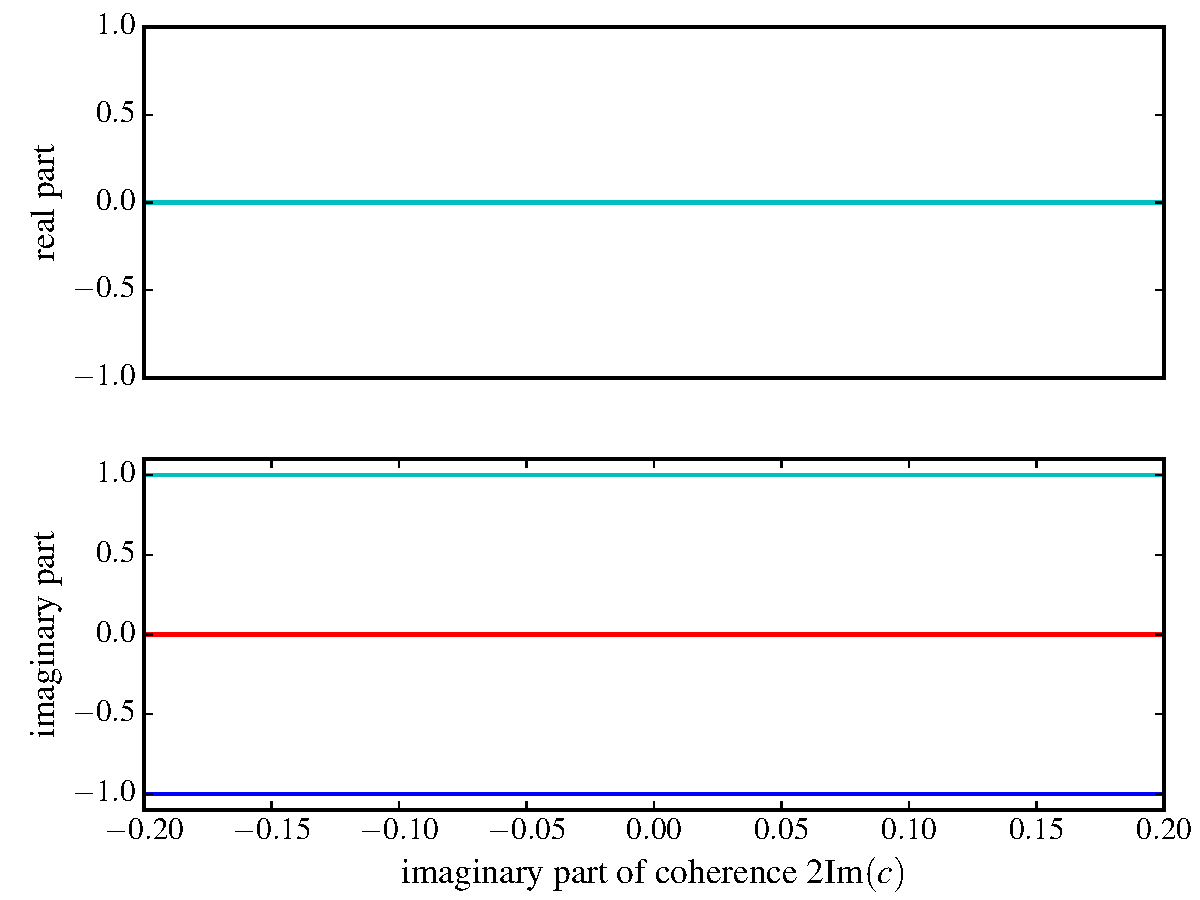
\includegraphics[width=0.7\textwidth]{figs/J1_eigenvalues_cVar_t1_0.004_m0.0.pdf}
	\caption{Variation of real and imaginary part of eigenvalues of $\mathbb{J}_1$ for varying imaginary part of coherence $2\mathrm{Im}(c)$ for $n=\frac{1}{2}$.}\label{fig:J1_cVar_m0}
\end{figure}

\begin{figure}[!h]
	\centering
	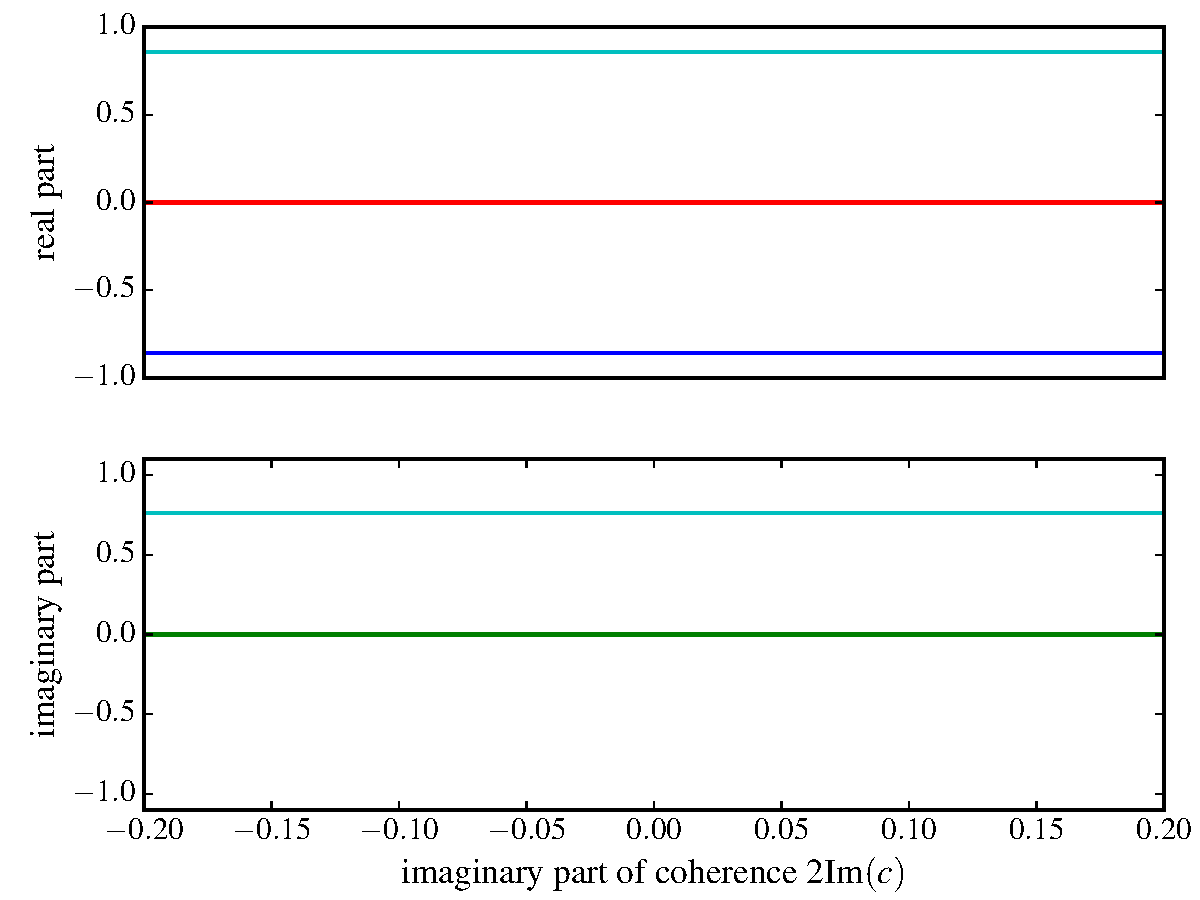
\includegraphics[width=0.7\textwidth]{figs/J1_eigenvalues_cVar_t1_0.004_m0.5.pdf}
	\caption{Variation of real and imaginary part of eigenvalues of $\mathbb{J}_1$ for varying imaginary part of coherence $2\mathrm{Im}(c)$ for $n=\frac{1}{4}$.}\label{fig:J1_cVar_m0.5}
\end{figure}
\clearpage
The Jacobian for the second family of fixed points $\xi_2$ reads
\begin{equation}
	\mathds{J}_2 =\begin{pmatrix}
		0 & -i(t_0+2t_1^2 c) & 0 & 0\\
		-2i(t_0+2t_1^2 c) & 0 & 0 & 0\\
		0 & 0 & 0 & 1 \\
		0 & -t_1 & -1 & 0
	\end{pmatrix}
\end{equation}
with $c$. Since at this fixed point the filling is fixed, the only free parameter is the coherence $c$, which is real. \Cref{fig:J2_cVar_m0.5} shows the real and imaginary parts of the spectrum of $\mathbb{J}_2$ as a function of coherence $c$. 
\begin{figure}[!h]
	\centering
	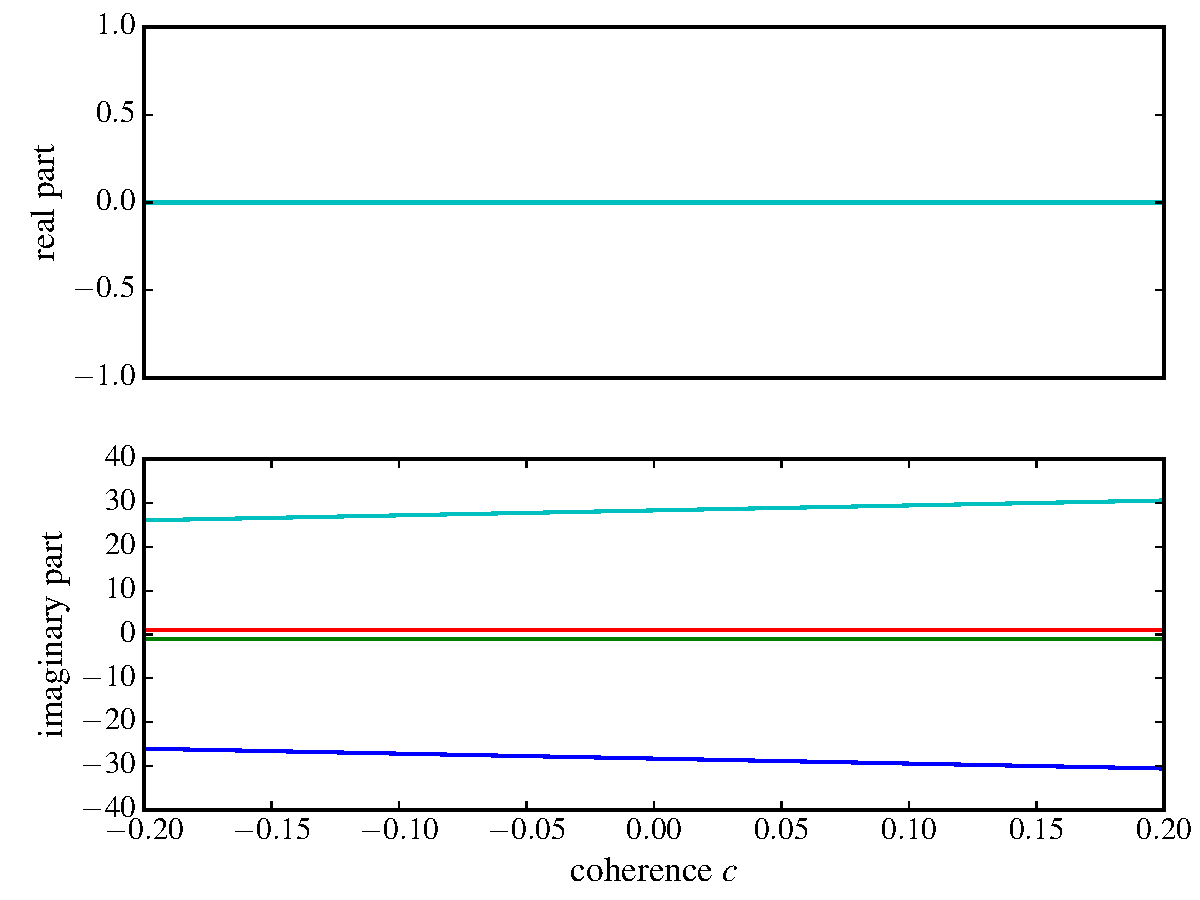
\includegraphics[width=0.7\textwidth]{figs/J2_eigenvalues_cVar_t1_0.004.pdf}
	\caption{Variation of real and imaginary part of eigenvalues of $\mathbb{J}_2$ for varying imaginary part of coherence $2\mathrm{Im}(c)$ for $n=\frac{1}{2}$.}\label{fig:J2_cVar_m0.5}
\end{figure}



\subsubsection{Open system}


\section{Solving the steady state in Ehrenfest-HEOM directly}
\clearpage
\section{Solving the vibrational relaxation problems using a classical vib. bath}
{\color{blue} Does a classical vibrational Ohmic bath lead to decoherence in the quantum subsystem?}

We consider a variation of the model considered before. The Hamiltonian of the molecule is now extended by including $m$ vibrational modes $X_{(k)}$ that couple to the $j$th bond vibration. The Hamiltonian reads
\begin{align*}
	H_\mathrm{sys} = H_\mathrm{el} + H_\mathrm{el-vib} + H_\mathrm{vib} + \sum_{j=1}^{N-1}\sum_{k=1}^m \left[ g_{k} X_j X_{(k)} + \frac{\omega_{(k)}}{2\hbar \omega} \left(X_{(k)}^2 + P_{(k)}^2 + \frac{1}{2}\right) \right]
\end{align*}
where $H_\mathrm{el},H_\mathrm{el-vib}$ and $H_\mathrm{vib}$ are as in the original Fransson model and the last term describes the coupling and the harmonic term of the additional harmonic modes. The molecule is coupled to two noninteracting fermionic leads in the same way as used in the previous reports.
We will call these additional degrees of freedom as "bath" degrees of freedom. Note that in this formulation used here, each system vibrational mode is coupled a common bath. This bath is characterized by its spectral density, 
\begin{equation*}
	J(\omega) = \pi\sum_j g_j^2 \delta(\hbar \omega-\hbar \omega_j) 
\end{equation*}
is assumed to be characterized by an Ohmic spectral density
\begin{equation*}
	J(\omega) = \frac{\pi\hbar}{2}\eta\omega \exP{-\frac{\omega}{\omega_c}}
\end{equation*}

Following Weiss (p. 19ff): 
\begin{align*}
	H &= H_S + H_R + H_I\\
	H_S &= \frac{p^2}{2M} + \frac{m\omega^2 q^2}{2} \\
	H_R &= \sum_\alpha \left(\frac{1}{2} \frac{p_\alpha^2}{m_\alpha} + \frac{1}{2}m_\alpha \omega_\alpha^2 x_\alpha^2 \right)\\
	H_I &= \sum_\alpha \left(-c_\alpha q x_\alpha + \frac{c_\alpha^2 q^2}{2m_\alpha \omega_\alpha^2} \right)
\end{align*}
and the classical equilibrium density of the unperturbed reservoir is 
\begin{equation*}
	\rho_R=Z^{-1} \exp\left\{-\beta \sum_\alpha \left(\frac{p_\alpha^2}{2m_\alpha} + \frac{m_\alpha \omega_\alpha^2}{2}x_\alpha^2\right)\right\}.
\end{equation*}
Transforming the coordinates and momenta according to 
\begin{equation}
	\hat{X}_j = \sqrt{\frac{m_j\omega_j}{\hbar}} \hat{x}_j, \qquad \hat{P}_j = \frac{\hat{p}_j}{\sqrt{\hbar m_j\omega_j}}
\end{equation}
one finds the Hamiltonian to be 
\begin{align*}
	H_S &= \frac{\hbar \omega}{2}\left(X^2 + P^2 + \frac{1}{2}\right) \\
	H_R &= \sum_\alpha \frac{\hbar \omega_\alpha}{2} \left(X_\alpha^2  + P_\alpha^2 + \frac{1}{2}\right)\\
	H_I &= \sum_\alpha \left(-\frac{\hbar}{\sqrt{m_\alpha \omega_\alpha m\omega}}c_\alpha X X_\alpha + \frac{\hbar}{m \omega}\frac{c_\alpha^2 X^2}{2m_\alpha \omega_\alpha^2} \right)
\end{align*}
For example, in this paper \cite{kab2004statistical}, the Hamiltonian reads
\begin{align*}
	H_S &= \frac{\hbar \omega}{2}\left(X^2 + P^2 + \frac{1}{2}\right) \\
	H_R &= \sum_\alpha \frac{\hbar \omega_\alpha}{2} \left(X_\alpha^2  + P_\alpha^2 + \frac{1}{2}\right)\\
	H_I &= \sum_\alpha \left(-\frac{\hbar}{\sqrt{m_\alpha \omega_\alpha m\omega}}c_\alpha X X_\alpha + \frac{\hbar}{m \omega}\frac{c_\alpha^2 X^2}{2m_\alpha \omega_\alpha^2} \right)
\end{align*}
The Ehrenfest equations of motion for the vibrational degrees of freedom are
\begin{align*}
	\dot{X}_j &= P_j \\
	\dot{P}_j &= -\tr{\rho(t)\partial_{X_j} H}  \\
	\dot{X}_{(k)} &= P_{(k)} \\
	\dot{P}_{(k)} &= \sum_j \frac{1}{\sqrt{m_{(k)}\omega_{(k)} m\omega^3}}c_{(k)} X_j 
\end{align*}

\printbibliography
\end{document}


